\chapter{BİLGİ GÜVENLİĞİ VE VERİ KORUMA}

\section*{Giriş}
Bilgi güvenliği, bir kuruluşun en değerli varlıklarından biri olan bilgiyi korumaya odaklanan stratejik bir alandır. Bu koruma, yalnızca teknik önlemlerle sınırlı kalmayıp, aynı zamanda yönetimsel ve fi kontrolleri de içerir. Bilgi güvenliğinin temelini oluşturan ve uluslararası alanda kabul görmüş ilkeler ve kavramlar, bu alanda uzmanlaşmak isteyen her profesyonel için kritik öneme sahiptir.

\section{Bilgi Güvenliğinin Temel Kavramları ve İlkeleri}

\subsection{CIA Triad: Gizlilik (Confidentiality), Bütünlük (Integrity), Kullanılabilirlik (Availability)}

CIA Triad, bilgi güvenliğinin temelini oluşturan üç ana unsuru ifade eder ve güvenli bir sistemin yapı taşlarını oluşturur. Bu üç unsur, birbirinden bağımsız düşünülemeyen ve birbirini tamamlayan bir bütündür.

\begin{itemize}
    \item \textbf{Gizlilik (Confidentiality):} Bu ilke, bilginin yalnızca yetkili kişiler tarafından erişilebilir olmasını sağlamayı amaçlar. Yetkisiz kişilerin hassas verilere erişimini engellemek için şifreleme, erişim kontrol listeleri ve veri sınıflandırma gibi yöntemler kullanılır. Gizlilik ihlali, kredi kartı bilgileri veya kişisel olarak tanımlanabilir bilgilerin (PII) çalınması gibi saldırılarla gerçekleşebilir. Bilginin doğru kişilere, izin, resmi erişim onayı ve bilme ihtiyacı (need-to-know) prensiplerine uygun olarak sunulması esastır.
    \item \textbf{Bütünlük (Integrity):} Bütünlük, bilginin yetkisiz kişiler tarafından değiştirilmemesi, doğruluğunun, eksiksizliğinin ve güvenilirliğinin korunması anlamına gelir. İki temel bütünlük türü bulunmaktadır: veri bütünlüğü ve sistem bütünlüğü. Veri bütünlüğü, bilgilerin yetkisiz değişikliklere karşı korunmasını hedeflerken, sistem bütünlüğü sunucular, ağ cihazları ve uygulamalar gibi bir sistemin kendisinin yetkisiz değişikliklerden korunmasını amaçlar. Bir dosya üzerinde kimin, ne zaman, hangi değişikliği yaptığının kayıt altına alınması, bütünlüğün sağlanması için kritik bir adımdır.
    \item \textbf{Kullanılabilirlik (Availability):} Bu ilke, yetkili kullanıcıların ihtiyaç duydukları anda bilgiye ve sistemlere kesintisiz bir şekilde erişebilmesini ifade eder. Bir sistemin çökmesi veya bir siber saldırı sonucu hizmet verememesi durumunda, kullanılabilirlik ilkesi ihlal edilmiş olur. Yedekleme sistemleri, saldırı önleme çözümleri ve iyi planlanmış bir altyapı, kullanılabilirliğin güvence altına alınması için zorunludur.
\end{itemize}

Bu üç unsur arasındaki ilişki, tek birinin ihlalinin diğerlerini de olumsuz etkileyebilmesiyle yakından ilişkilidir. Örneğin, bir Dağıtılmış Hizmet Engelleme (DDoS) saldırısı doğrudan kullanılabilirlik ilkesini hedef alırken, bir siber saldırganın veritabanına sızarak hem müşteri bilgilerini çalması (gizlilik ihlali) hem de bu verileri değiştirmesi (bütünlük ihlali), ardından da veritabanı sunucusunun çökmesine neden olması (kullanılabilirlik ihlali) tüm triad'ın tehlikeye girdiğini gösterir. Bu örnek, bilgi güvenliğinin bir bütün olarak ele alınması gerektiğini ve güvenlik zincirinin en zayıf halkası koptuğunda tüm sistemin savunmasız kalabileceğini ortaya koymaktadır.

Bu üç temel unsurun yanı sıra, modern güvenlik yaklaşımları ek kavramları da temel bileşenler olarak kabul etmektedir. Kimlik doğrulama (Authentication), Yetkilendirme (Authorization) ve İnkâr Edilemezlik (Non-repudiation) gibi ilkeler, CIA üçlüsünü tamamlayarak daha sağlam bir güvenlik duruşu oluşturur. Kimlik doğrulama, bilgiye erişim talep eden kullanıcının kimliğinin doğrulanmasını sağlarken, yetkilendirme kullanıcının sistemde ne yapabileceğini belirler. İnkâr edilemezlik ise, bir işlemin veya olayın kaynağının ispatlanabilirliğini sağlayarak ilgili kişilerin bu olayı reddedememesini garanti eder. Bu ek unsurlar, güvenlik kontrol mekanizmalarının sadece veri üzerinde değil, aynı zamanda kullanıcılar ve süreçler üzerinde de yoğunlaşması gerektiğini gösterir.

\subsection{Bilgi Güvenliği Risk Yönetimi ve Metodolojileri}

Bilgi güvenliği risk yönetimi, bir kuruluşun bilgi varlıklarını koruma amacıyla potansiyel tehditleri, zafiyetleri ve bunların yaratabileceği etkileri sistematik bir şekilde ele alan bir süreçtir. Etkili bir risk yönetimi programı, riskleri en aza indirmek ve iş sürekliliğini sağlamak için stratejik kararlar alınmasına yardımcı olur. Modern risk yönetimi, çeşitli metodolojiler ve çerçeveler kullanılarak uygulanır:

\begin{itemize}
\item \textbf{CTEM (Continuous Threat Exposure Management) Metodolojisi:} Sürekli tehdit risklerini izlemeye ve yönetmeye odaklanan bir yaklaşımdır. Beş ana aşamadan oluşur:
\begin{enumerate}
    \item \textbf{Kapsam (Scope):} Risk değerlendirmesi için önceliklendirilen alanların belirlenmesi
    \item \textbf{Değerlendirme (Assess):} Belirlenen alandaki tehditlerin ve risklerin analizi
    \item \textbf{Mobilizasyon (Mobilize):} Risk azaltma planlarının geliştirilmesi ve kaynakların tahsisi
    \item \textbf{Doğrulama (Validate):} Alınan önlemlerin etkinliğinin test edilmesi
    \item \textbf{İzleme (Monitor):} Sürekli izleme ve yeni tehditlerin tespiti
\end{enumerate}

\item \textbf{FAIR (Factor Analysis of Information Risk):} Siber riskleri finansal terimlerle ölçmeye odaklanan bir metodoloji. FAIR, risk analizini kantitatif hale getirerek, risk yönetimi kararlarının daha objektif ve veri odaklı olmasını sağlar. Temel bileşenleri:
\begin{itemize}
    \item Risk = Olasılık x Etki formülünü detaylandırır
    \item Kayıp Olayı Sıklığı (LEF - Loss Event Frequency)
    \item Kayıp Büyüklüğü (LM - Loss Magnitude)
    \item Risk skorlarını finansal değerlere dönüştürme
\end{itemize}

\item \textbf{OCTAVE (Operationally Critical Threat, Asset, and Vulnerability Evaluation):} Operasyonel hedeflere dayalı bir risk değerlendirme çerçevesidir. Üç ana fazdan oluşur:
\begin{enumerate}
    \item \textbf{Organizasyonel Görüş:} Varlıklar, tehditler ve mevcut güvenlik uygulamaları belirlenir
    \item \textbf{Teknoloji Görüşü:} Teknik zafiyetler analiz edilir
    \item \textbf{Strateji ve Plan Geliştirme:} Risk değerlendirme sonuçlarına göre güvenlik stratejisi oluşturulur
\end{enumerate}
\end{itemize}

Risk yönetiminin temel kavramları şunlardır:

\begin{itemize}
    \item \textbf{Tehdit:} Bir sistemin zafiyetini kullanarak zarara yol açma potansiyeli taşıyan bir olay veya durumdur. Örnek olarak kötü amaçlı yazılımlar, doğal afetler veya kötü niyetli insiderlar verilebilir.
    \item \textbf{Zafiyet:} Bir sistemdeki, ağdaki veya uygulamadaki güvenlik açığı veya zayıflıktır. Örneğin, yama yapılmamış bir işletim sistemi veya zayıf parola politikaları bir zafiyet oluşturur.
    \item \textbf{Risk:} Bir tehdidin bir zafiyeti kullanarak bir varlığa zarar verme olasılığı ve potansiyel etkisidir. Risk, genellikle şu formülle hesaplanır:
\end{itemize}

$$\text{Risk} = \text{Tehdit Etkisi} \times \text{Olasılık}$$

\begin{itemize}
    \item \textbf{Etki:} Bir riskin gerçekleşmesi durumunda ortaya çıkacak zararın boyutu ve ciddiyetidir. Bu zarar, finansal kayıplar, itibar zedelenmesi veya yasal yaptırımlar şeklinde olabilir.
\end{itemize}

\textbf{Pratik Örnek Senaryo: Web Uygulaması Risk Analizi}

Bir e-ticaret şirketinin, SQL Enjeksiyonu saldırılarına karşı müşteri veritabanı güvenliğini değerlendirdiği bir risk analizi senaryosu aşağıda adım adım incelenmiştir.

\begin{enumerate}
    \item \textbf{Varlık Tanımlama:} Korunması gereken en kritik varlık, müşteri adı, adresi, kredi kartı bilgileri ve sipariş geçmişi gibi hassas verileri içeren müşteri veritabanıdır.
    \item \textbf{Tehdit Tanımlama:} Potansiyel tehdit, bir siber saldırganın web uygulamasındaki bir zafiyeti kullanarak veritabanına erişim sağlamasıdır.
    \item \textbf{Zafiyet Tanımlama:} Web uygulamasının, kullanıcıdan gelen girdileri yeterince filtrelemeden doğrudan veritabanı sorgusunda kullanması, bir SQL Enjeksiyonu zafiyetine yol açmaktadır.
    \item \textbf{Etki Değerlendirmesi:} Bu zafiyetin kullanılmasıyla ortaya çıkabilecek etkiler:
    \begin{itemize}
        \item Müşteri verilerinin çalınması: Şirketin itibarına büyük zarar verir ve yasal para cezalarına yol açar. \textbf{(Etki: Çok Yüksek)}
        \item Veri manipülasyonu: Yanlış sipariş bilgileri veya finansal veriler, iş süreçlerini aksatır. \textbf{(Etki: Yüksek)}
    \end{itemize}
    \item \textbf{Olasılık Değerlendirmesi:} Saldırganların SQL Enjeksiyonu yöntemini yaygın olarak kullandığı ve web uygulamasının aktif olarak internete açık olduğu göz önüne alındığında, bu zafiyetin istismar edilme olasılığı \textbf{(Olasılık: Yüksek)} olarak değerlendirilir.
    \item \textbf{Risk Hesaplaması:} Yukarıdaki formüle göre: `Risk = Çok Yüksek Etki x Yüksek Olasılık = Çok Yüksek Risk`.
\end{enumerate}

Bu analiz, şirketin bu riski acilen ele alması ve zafiyeti gidermesi gerektiğini gösterir. Risk yönetimi metodolojileri, bu tür analizleri sistematik bir şekilde yaparak güvenlik programlarının temelini oluşturur. Öte yandan, risk yönetimi artık statik, bir defalık bir görev olmaktan çıkıp, sürekli izlenmesi ve düzeltilmesi gereken dinamik bir süreç haline gelmiştir. Risk yönetimi göstergeleri (KPI'lar), risk maruziyetini ölçmek ve risk azaltma çabalarının etkinliğini değerlendirmek için kullanılır. Bu durum, siber güvenlik programlarının durağan "kurallara dayalı" yaklaşımlar yerine, sürekli iyileştirme ve adaptasyon gerektiren "risk tabanlı" bir modele dönüştüğünü ortaya koymaktadır.

\subsection{Güvenlik Görevleri Ayrılığı (Segregation of Duties)}

Güvenlik Görevleri Ayrılığı (SoD), bir kritik işlemin baştan sona tek bir kişi veya entity tarafından tamamlanmasını engelleyen temel bir güvenlik prensibidir. Bu ilkenin temel amacı, içeriden kaynaklanan kötüye kullanımı ve dolandırıcılığı, birden fazla kişinin iş birliği olmadan neredeyse imkansız hale getirmektir. SoD, sistemlerin gizliliğini, bütünlüğünü ve kullanılabilirliğini korumak için tasarlanmış bir kontrol mekanizmasıdır.

Teorik olarak basit bir fikir olmasına rağmen, SoD'nin pratikteki uygulaması, saldırıları yavaşlatan ve iç tehditleri önemli ölçüde azaltan bir dizi kontrol noktası oluşturur.

\textbf{Pratik Uygulama Örnekleri:}

\begin{itemize}
    \item \textbf{Sistem Yönetimi:} Bir sistem yöneticisinin, bir sistemde hem kullanıcı hesabı oluşturma, hem bu hesaba ayrıcalık verme hem de bu işlemlerin izlendiği denetim kayıtlarını silme yetkisine sahip olması en yüksek riski taşır. Etkili bir SoD modeli, hesap oluşturma görevini bir yöneticiye, log izleme ve denetleme görevini ise bir başka role atar. Bu ayrım, hataların ve kötü niyetli değişikliklerin fark edilmesini kolaylaştırır.
    \item \textbf{Ağ Güvenliği:} Eğer bir ağ mühendisi hem güvenlik duvarı kurallarını yazma hem de bunları onaylama yetkisine sahipse, sisteme arka kapı (backdoor) yerleştirmesi ve bunu fark edilmeden yapması riski doğar. SoD ilkesi, bir kişinin kuralı oluşturmasını, bir diğerinin bu kuralı gözden geçirmesini ve bir güvenlik yöneticisinin de son onayı vermesini gerektirerek bu riski ortadan kaldırır.
    \item \textbf{Yazılım Geliştirme:} Bir geliştiricinin, kodunu doğrudan canlı (production) ortama geçirmesini önlemek için, kodun yazılması, test edilmesi ve canlıya alınması görevleri farklı kişilere veya ekiplere atanır. Bu sayede, güvenlik açığı içeren veya test edilmemiş kodların kritik sistemlere ulaşması engellenir.
\end{itemize}

SoD, HIPAA, SOX, GDPR ve ISO 27001 gibi düzenleyici çerçeveler için temel bir gerekliliktir. Metinlerde bahsedilen, bir hastanenin HIPAA denetimini, bir teknisyenin hem kullanıcı ekleyebilmesi hem de izleme sistemlerini devre dışı bırakabilmesi nedeniyle geçememesi örneği, bu ilkenin yasal zorunluluklardaki somut yansımasını gözler önüne serer. SoD, aynı zamanda "en az ayrıcalık" (least privilege) ve "ihtiyaç duyulduğu kadar bilme" (need-to-know) ilkelerinin bir uzantısıdır; bir kullanıcıya görevini tamamlaması için sadece gerekli yetkileri vermek ve bu yetkileri kritik bir sürecin tek bir aşamasına sınırlamak, iç tehditlere karşı güçlü bir savunma hattı oluşturur.

\subsection{Savunma Derinliği (Defense-in-Depth) Stratejisi}

Savunma Derinliği (DiD), bir kuruluşu korumak için birden fazla güvenlik önlemini bir arada kullanan kapsamlı bir siber güvenlik stratejisidir. Bu strateji, bir savunma hattı aşılırsa, ek katmanların tehdidi durdurmasını sağlamayı amaçlar. Bu yaklaşım, askeri bir stratejiden ilham alır ve bir orta çağ kalesinin çok katmanlı savunmasına benzetilir. Saldırganın hendek, kale kapısı ve surlar gibi birden fazla engeli aşması gerektiği gibi, siber saldırganların da bir dizi güvenlik kontrolünden geçmesi gerekir.

DiD stratejisinin üç ana katmanı bulunmaktadır:

\begin{itemize}
    \item \textbf{Yönetimsel (Administrative) Kontroller:} Bunlar, bir kuruluşun güvenlik politikalarını, prosedürlerini ve süreçlerini içerir. Örnekler arasında risk değerlendirmeleri, çalışan güvenlik eğitimleri, erişim kontrol politikaları ve olay müdahale planları yer alır.
    \item \textbf{Fiziksel (Physical) Kontroller:} Bu katman, fiziksel varlıklara ve BT sistemlerine yetkisiz erişimi önlemeyi amaçlar. Kilitli sunucu odaları, güvenlik kameraları, giriş kartları ve güvenlik görevlileri bu kategoriye girer.
    \item \textbf{Teknik (Technical) Kontroller:} En karmaşık katman olan teknik kontroller, donanım ve yazılım tabanlı çözümleri içerir. Bu çözümler arasında güvenlik duvarları, antivirüs yazılımları, saldırı tespit/önleme sistemleri (IDS/IPS), şifreleme ve yedekleme sistemleri bulunur.
\end{itemize}

\textbf{Modern Savunma Derinliği Stratejileri}

Tarihsel olarak, savunma derinliği stratejileri, geleneksel çevre tabanlı (perimeter-based) güvenlik modelleri etrafında şekillenmiştir; bu modeller, bir ağın çevresini korumaya odaklanır. Ancak, dijital dönüşüm, uzaktan çalışma ve bulut hizmetlerinin yaygınlaşması, geleneksel "güvenilir ağ" kavramını ortadan kaldırmıştır. Bu yeni ortamda, saldırganların zaten ağın içinde olduğu varsayımıyla hareket eden bir "Sıfır Güven" (Zero Trust) yaklaşımı benimsenmiştir. Bu stratejide, her erişim talebi sürekli olarak doğrulanır ve yetkilendirilir.

Modern DiD stratejisi, geleneksel kontrolleri (güvenlik duvarı, antivirüs) yeni çözümlerle birleştirir:

\begin{itemize}
    \item \textbf{Ayrıcalıklı Erişim Yönetimi (PAM):} Süper kullanıcılar ve etki alanı yöneticileri gibi yüksek ayrıcalıklı hesaplara erişimi izler ve güvence altına alır.
    \item \textbf{Uç Nokta Ayrıcalık Yönetimi (EPM):} Tüm uç noktalarda ayrıcalıklı erişimi kısıtlar, yanal hareketi (lateral movement) engeller ve fidye yazılımı gibi kötü amaçlı yazılımlara karşı koruma sağlar.
    \item \textbf{Uyarlanabilir Çok Faktörlü Kimlik Doğrulama (MFA):} Kullanıcının konumu, saati veya cihaz türü gibi bağlamsal bilgilere göre kimlik doğrulama faktörlerinin uygulanmasını sağlar.
\end{itemize}

Bu yeni yaklaşım, bir güvenlik stratejisinin, değişen teknolojik ve operasyonel koşullara nasıl adapte olması gerektiğini gösteren önemli bir evrimdir. Saldırganların birincil savunma hattını aşması durumunda, iç mekanizmaların onları durdurması beklenir. Bu çok katmanlı ve sürekli doğrulama yaklaşımı, tek bir kontrol noktasının başarısızlığının tüm sistemi riske atmasını önler.

\subsection{Need-to-Know ve Least Privilege Prensipleri}

En Az Ayrıcalık (Least Privilege) ve İhtiyaç Duyulduğu Kadar Bilme (Need-to-Know) ilkeleri, siber güvenlikte erişim kontrolünü yöneten iki temel prensiptir. Her ikisi de risk azaltmayı hedefler, ancak farklı odak noktaları vardır.

\begin{itemize}
    \item \textbf{En Az Ayrıcalık (Least Privilege):} Bu ilke, bir kullanıcının, programın veya sürecin, görevini yerine getirmek için gereken minimum erişim yetkisine sahip olması gerektiğini belirtir. Bu, bir çalışanın işini yapmak için sadece gerekli olan yetkileri alması ve fazlasına sahip olmaması anlamına gelir. Örneğin, bir veritabanına veri girmekle görevli bir kullanıcı, bu verileri silme veya veritabanı şemasını değiştirme yetkisine sahip olmamalıdır. Bu prensip, kötüye kullanımdan veya yanlışlıkla yapılan hatalardan kaynaklanabilecek potansiyel zararı en aza indirmeyi amaçlar.
    \item \textbf{İhtiyaç Duyulduğu Kadar Bilme (Need-to-Know):} Bu ilke, bir kullanıcının, işini tamamlamak için bilmesi veya erişmesi gereken bilgiye sadece o anda erişiminin olması gerektiğini vurgular. Bu prensip, gizli bilgilerin yayılmasını kısıtlamak için kullanılır ve en az ayrıcalık ilkesini tamamlar. En az ayrıcalık \textbf{ne yapabileceğine} odaklanırken, ihtiyaç duyulduğu kadar bilme \textbf{neye erişebileceğine} odaklanır ve daha spesifiktir.
\end{itemize}

Bu ilkelerin güvenlik ve operasyonel açıdan birçok faydası bulunmaktadır:
\begin{itemize}
    \item \textbf{Azaltılmış Risk:} Düşük ayrıcalıklı bir hesabın ele geçirilmesi durumunda, saldırganın sistemi genelinde yayılabileceği etki alanı sınırlı kalır. Edward Snowden'ın, en üst görevi veritabanı yedeklemesi almak olmasına rağmen, yönetici ayrıcalıkları sayesinde milyonlarca gizli dosyayı sızdırabilmesi, bu ilkenin neden bu kadar kritik olduğunu gösteren çarpıcı bir örnektir.
    \item \textbf{Artırılmış Stabilite:} Sistemlere ve uygulamalara yapılan yetkisiz veya yanlışlıkla yapılan değişikliklerin etkisi, bu ilkelerle sınırlanır.
    \item \textbf{Geliştirilmiş Denetlenebilirlik:} Denetim süreçleri, sistemin en az ayrıcalık ilkesine göre tasarlandığı durumlarda daha kolay ve daha hızlı yürütülebilir.
\end{itemize}

\textbf{Pratik Uygulama Örnekleri}

Bu ilkelerin pratikte uygulanması, hem işletim sistemleri düzeyinde hem de merkezi yönetim araçları kullanılarak gerçekleştirilir.

\textbf{Linux Sistemlerinde Uygulama (\texttt{chown} ve \texttt{chmod})}

Linux’ta dosya ve dizin erişimini yönetmek için \texttt{chown} ve \texttt{chmod} komutları kullanılır. \texttt{chown}, dosya sahipliğini ve grubunu belirlerken, \texttt{chmod} sahiplik grubuna ve diğer kullanıcılara yönelik okuma, yazma ve çalıştırma izinlerini ayarlar. Bu iki komutun birlikte kullanımı, en az ayrıcalık ilkesinin uygulanmasının temelini oluşturur.

\textbf{Senaryo:} Kritik bir yapılandırma dosyasına sadece belirli bir hizmet hesabının erişmesini sağlamak.

\begin{enumerate}
    \item \textbf{Dosya Sahipliğini Değiştirme:} Dosyanın sahipliğini, uygulamayı çalıştıran kullanıcıya (\texttt{service\_user}) ve gruba (\texttt{service\_group}) verin.
    \begin{verbatim}
    $ sudo chown service_user:service_group /etc/critical_app/config.yaml
    \end{verbatim}
    \item \textbf{Erişim Yetkilerini Kısıtlama:} Dosya için sadece sahibine okuma ve yazma (\texttt{6}) izni, diğer herkese ise hiçbir (\texttt{0}) izni verin.
    \begin{verbatim}
    $ sudo chmod 600 /etc/critical_app/config.yaml
    \end{verbatim}
    Bu komut, \texttt{config.yaml} dosyasını sadece \texttt{service\_user}'ın okuyup yazabilmesini, diğer kullanıcıların ise dosyaya erişimini tamamen engellemesini sağlar.
\end{enumerate}

\textbf{Özel İzinler ve Pratik Senaryolar}

Linux'ta SGID (\texttt{Set Group ID}) ve Sticky Bit gibi özel izinler, en az ayrıcalık prensibini daha detaylı uygulamak için kullanılır.

\begin{itemize}
    \item \textbf{SGID} (\texttt{chmod 2xxx}): Bir dizine SGID izni verildiğinde, o dizin içinde oluşturulan yeni dosyalar, dizinin grubuna ait olur. Bu, paylaşılan bir çalışma dizininde çalışan farklı kullanıcıların, dosyaların sahipliğini ve yetkilerini korumasına yardımcı olur.
    \begin{verbatim}
$ sudo chmod 2775 /shared/project_dir
    \end{verbatim}
    \item \textbf{Sticky Bit} (\texttt{chmod 1xxx}): Bir dizine Sticky Bit izni verildiğinde, dizin içindeki dosyalar sadece kendi sahipleri, dizin sahibi veya \texttt{root} kullanıcısı tarafından silinebilir. Bu, özellikle \texttt{tmp} dizini gibi herkesin dosya oluşturabildiği ortak alanlarda yanlışlıkla veya kötü niyetli silmeleri önler.
    \begin{verbatim}
$ sudo chmod 1777 /tmp
    \end{verbatim}
\end{itemize}

\textbf{Windows Ortamında Uygulama}

Windows sistemlerinde, yerel yönetici haklarının merkezi olarak yönetimi, Grup İlkesi (Group Policy) aracılığıyla yapılır. Bu, "ayrıcalık kayması" (privilege creep) olarak bilinen ve bir kullanıcının zamanla artan yetkileri nedeniyle gereksiz riskler biriktirmesini önlemeye yardımcı olur.

\textbf{Adım Adım Yönetim Süreci:}

\begin{enumerate}
    \item \textbf{GPO Oluşturma:} Active Directory'de, yerel yönetici haklarını kaldırmak için bir Grup İlkesi Nesnesi (GPO) oluşturulur.
    \item \textbf{Politikayı Yapılandırma:} GPO düzenleme penceresinde \\
    \texttt{Computer Configuration > Preferences > Control Panel Settings > \\
    Local Users and Groups} yoluna gidilir.
    \item \textbf{Yerel Yöneticiler Grubunu Düzenleme:} Buradan, "Administrators" grubuna yeni bir kural eklenir. \texttt{Update} aksiyonu kullanılarak, belirlenen kullanıcılar hariç tüm kullanıcıların bu gruptan silinmesi sağlanır. Bu işlem, yerel yönetici yetkilerini şirket genelinde temizleyerek yalnızca onaylanmış hesapların bu gruba dahil olmasını sağlar.
\end{enumerate}

Pratikte, bazı eski veya kötü kodlanmış uygulamalar yönetici hakları olmadan çalışmayabilir. Bu tür durumlar için, kullanıcıya sürekli yönetici yetkisi vermek yerine, "just-in-time" (tam zamanında) ayrıcalıklar veren veya belirli uygulamalara anlık ayrıcalık yükseltme yetkisi tanıyan özel yazılımlar kullanılabilir. Bu çözümler, en az ayrıcalık ilkesini ihlal etmeden, çalışanların üretkenliğini sürdürmesine olanak tanır.

Bu prensiplerin uygulanması, teorik bir kavramdan pratik bir zorunluluğa dönüşen bir süreci temsil eder. İlk olarak bir olayı tanımlayan teorik kavramlar, Snowden sızıntıları gibi gerçek dünya örnekleri ile önem kazanmıştır. Bu önemin anlaşılması, eski uygulamalar gibi pratik zorlukları beraberinde getirmiş, bu zorluklar ise "just-in-time" erişim veya özel ayrıcalık yönetimi araçları gibi daha gelişmiş çözümlerin ortaya çıkmasını sağlamıştır. Bu dönüşüm, bir güvenlik ilkesinin, gerçek dünya sorunlarına yanıt olarak nasıl evrildiğinin ve bu evrimin yeni teknolojileri ve yönetim yaklaşımlarını nasıl doğurduğunun bir göstergesidir.

\section{Bilgi Güvenliği Standartları ve Framework'ler}

Bilgi güvenliği standartları ve çerçeveleri, bir kuruluşun bilgi varlıklarını etkili bir şekilde yönetmesi ve koruması için rehberlik sağlar. Bu çerçeveler, en iyi uygulamaları tanımlar ve denetlenebilir bir yapı sunar.

\subsection{ISO 27001/27002 Information Security Management}

ISO 27001, bir kuruluşun Bilgi Güvenliği Yönetim Sistemini (BGYS) kurması, uygulaması, sürdürmesi ve sürekli iyileştirmesi için gereklilikleri belirleyen uluslararası bir standarttır. Bu standart, bilgi güvenliğini yönetmeye yönelik risk tabanlı bir yaklaşım benimser. ISO 27001, gizlilik, bütünlük ve kullanılabilirlik ilkelerini benimseyerek bilginin güvenli bir şekilde yönetilmesini sağlamayı hedefler.

\begin{figure}[ht]
\centering
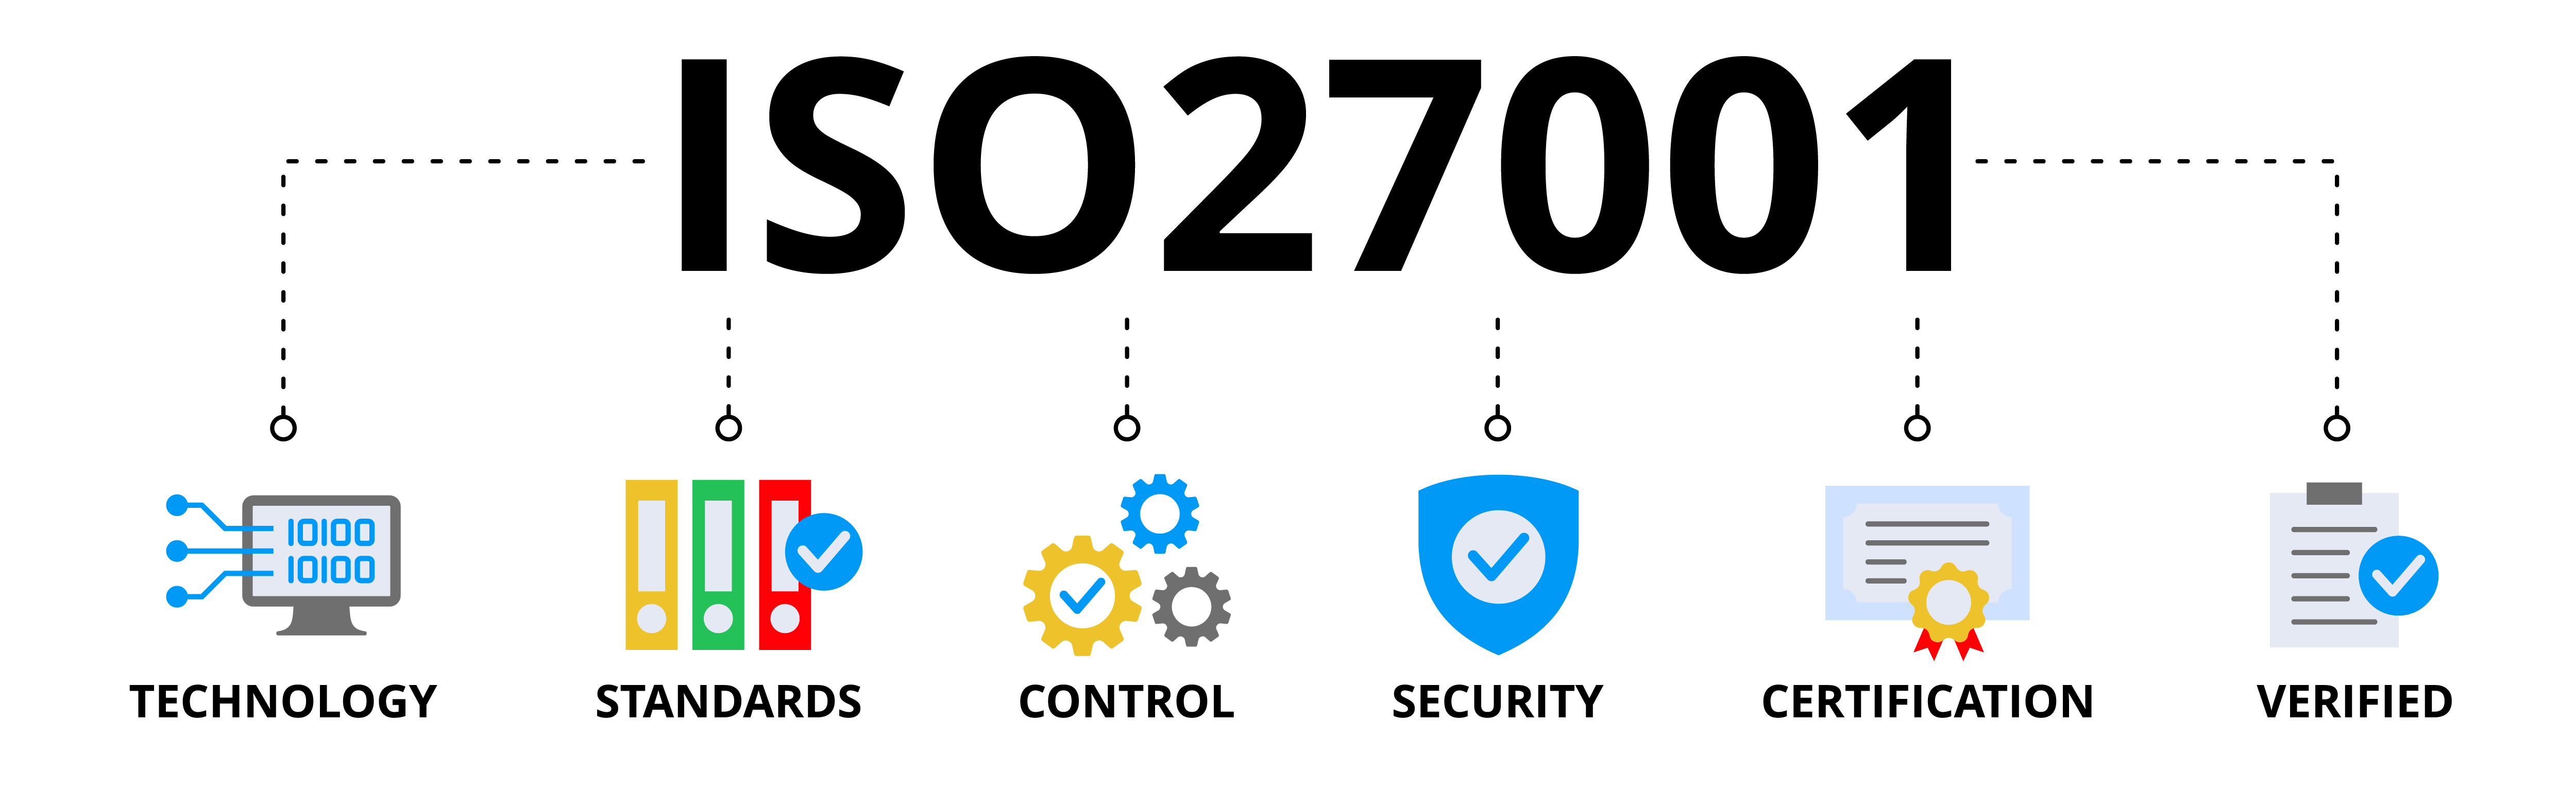
\includegraphics[width=0.6\textwidth]{img/ISO27001.png}
\caption{ISO 27001 Bilgi Güvenliği Yönetim Sistemi Standardı}
\label{fig:iso27001}
\end{figure}

ISO 27001'in en önemli özelliklerinden biri sertifikasyon sürecidir. Kuruluşlar, standartlara uygunluklarını kanıtlamak için harici bir denetçi tarafından kapsamlı bir yerinde denetime tabi tutulurlar. Denetimi geçen kuruluşlar, üç yıl geçerli olan bir ISO 27001 sertifikası alırlar. Bu sertifika, kuruluşun güvenliğe olan bağlılığını uluslararası düzeyde gösteren bir güven sinyalidir.

\subsection{NIST Cybersecurity Framework (CSF) Uygulamaları}

Ulusal Standartlar ve Teknoloji Enstitüsü (NIST) Siber Güvenlik Çerçevesi (CSF), siber güvenlik risklerini yönetmek ve azaltmak için kullanılan esnek bir rehberdir. Çerçeve, özellikle siber güvenlik programının ilk aşamalarında veya bir ihlali azaltmaya çalışırken kullanışlıdır ve daha teknik bir odak noktasına sahiptir. NIST CSF, beş ana işlevi etrafında yapılandırılmıştır:

\begin{itemize}
    \item \textbf{Tanımlama (Identify):} Sistemlerin, varlıkların, verilerin ve yeteneklerin siber güvenlik risklerini anlamak.
    \item \textbf{Koruma (Protect):} Kritik hizmetlerin sunumunu sağlamak için koruyucu önlemler almak.
    \item \textbf{Tespit Etme (Detect):} Siber güvenlik olaylarının zamanında tespit edilmesini sağlayan faaliyetleri uygulamak.
    \item \textbf{Müdahale Etme (Respond):} Bir olay tespit edildiğinde, etkilerini sınırlamak için bir plan dahilinde harekete geçmek.
    \item \textbf{Kurtarma (Recover):} Siber bir olaydan etkilenen işlevleri geri yüklemek ve iyileştirmek için planlar yapmak.
\end{itemize}

Bu beş işlev, NIST CSF'nin ana omurgasını oluşturur ve kuruluşlara risk yönetimi stratejilerini iş ihtiyaçlarıyla uyumlu hale getirme konusunda yardımcı olur.

\begin{figure}[H]
\centering
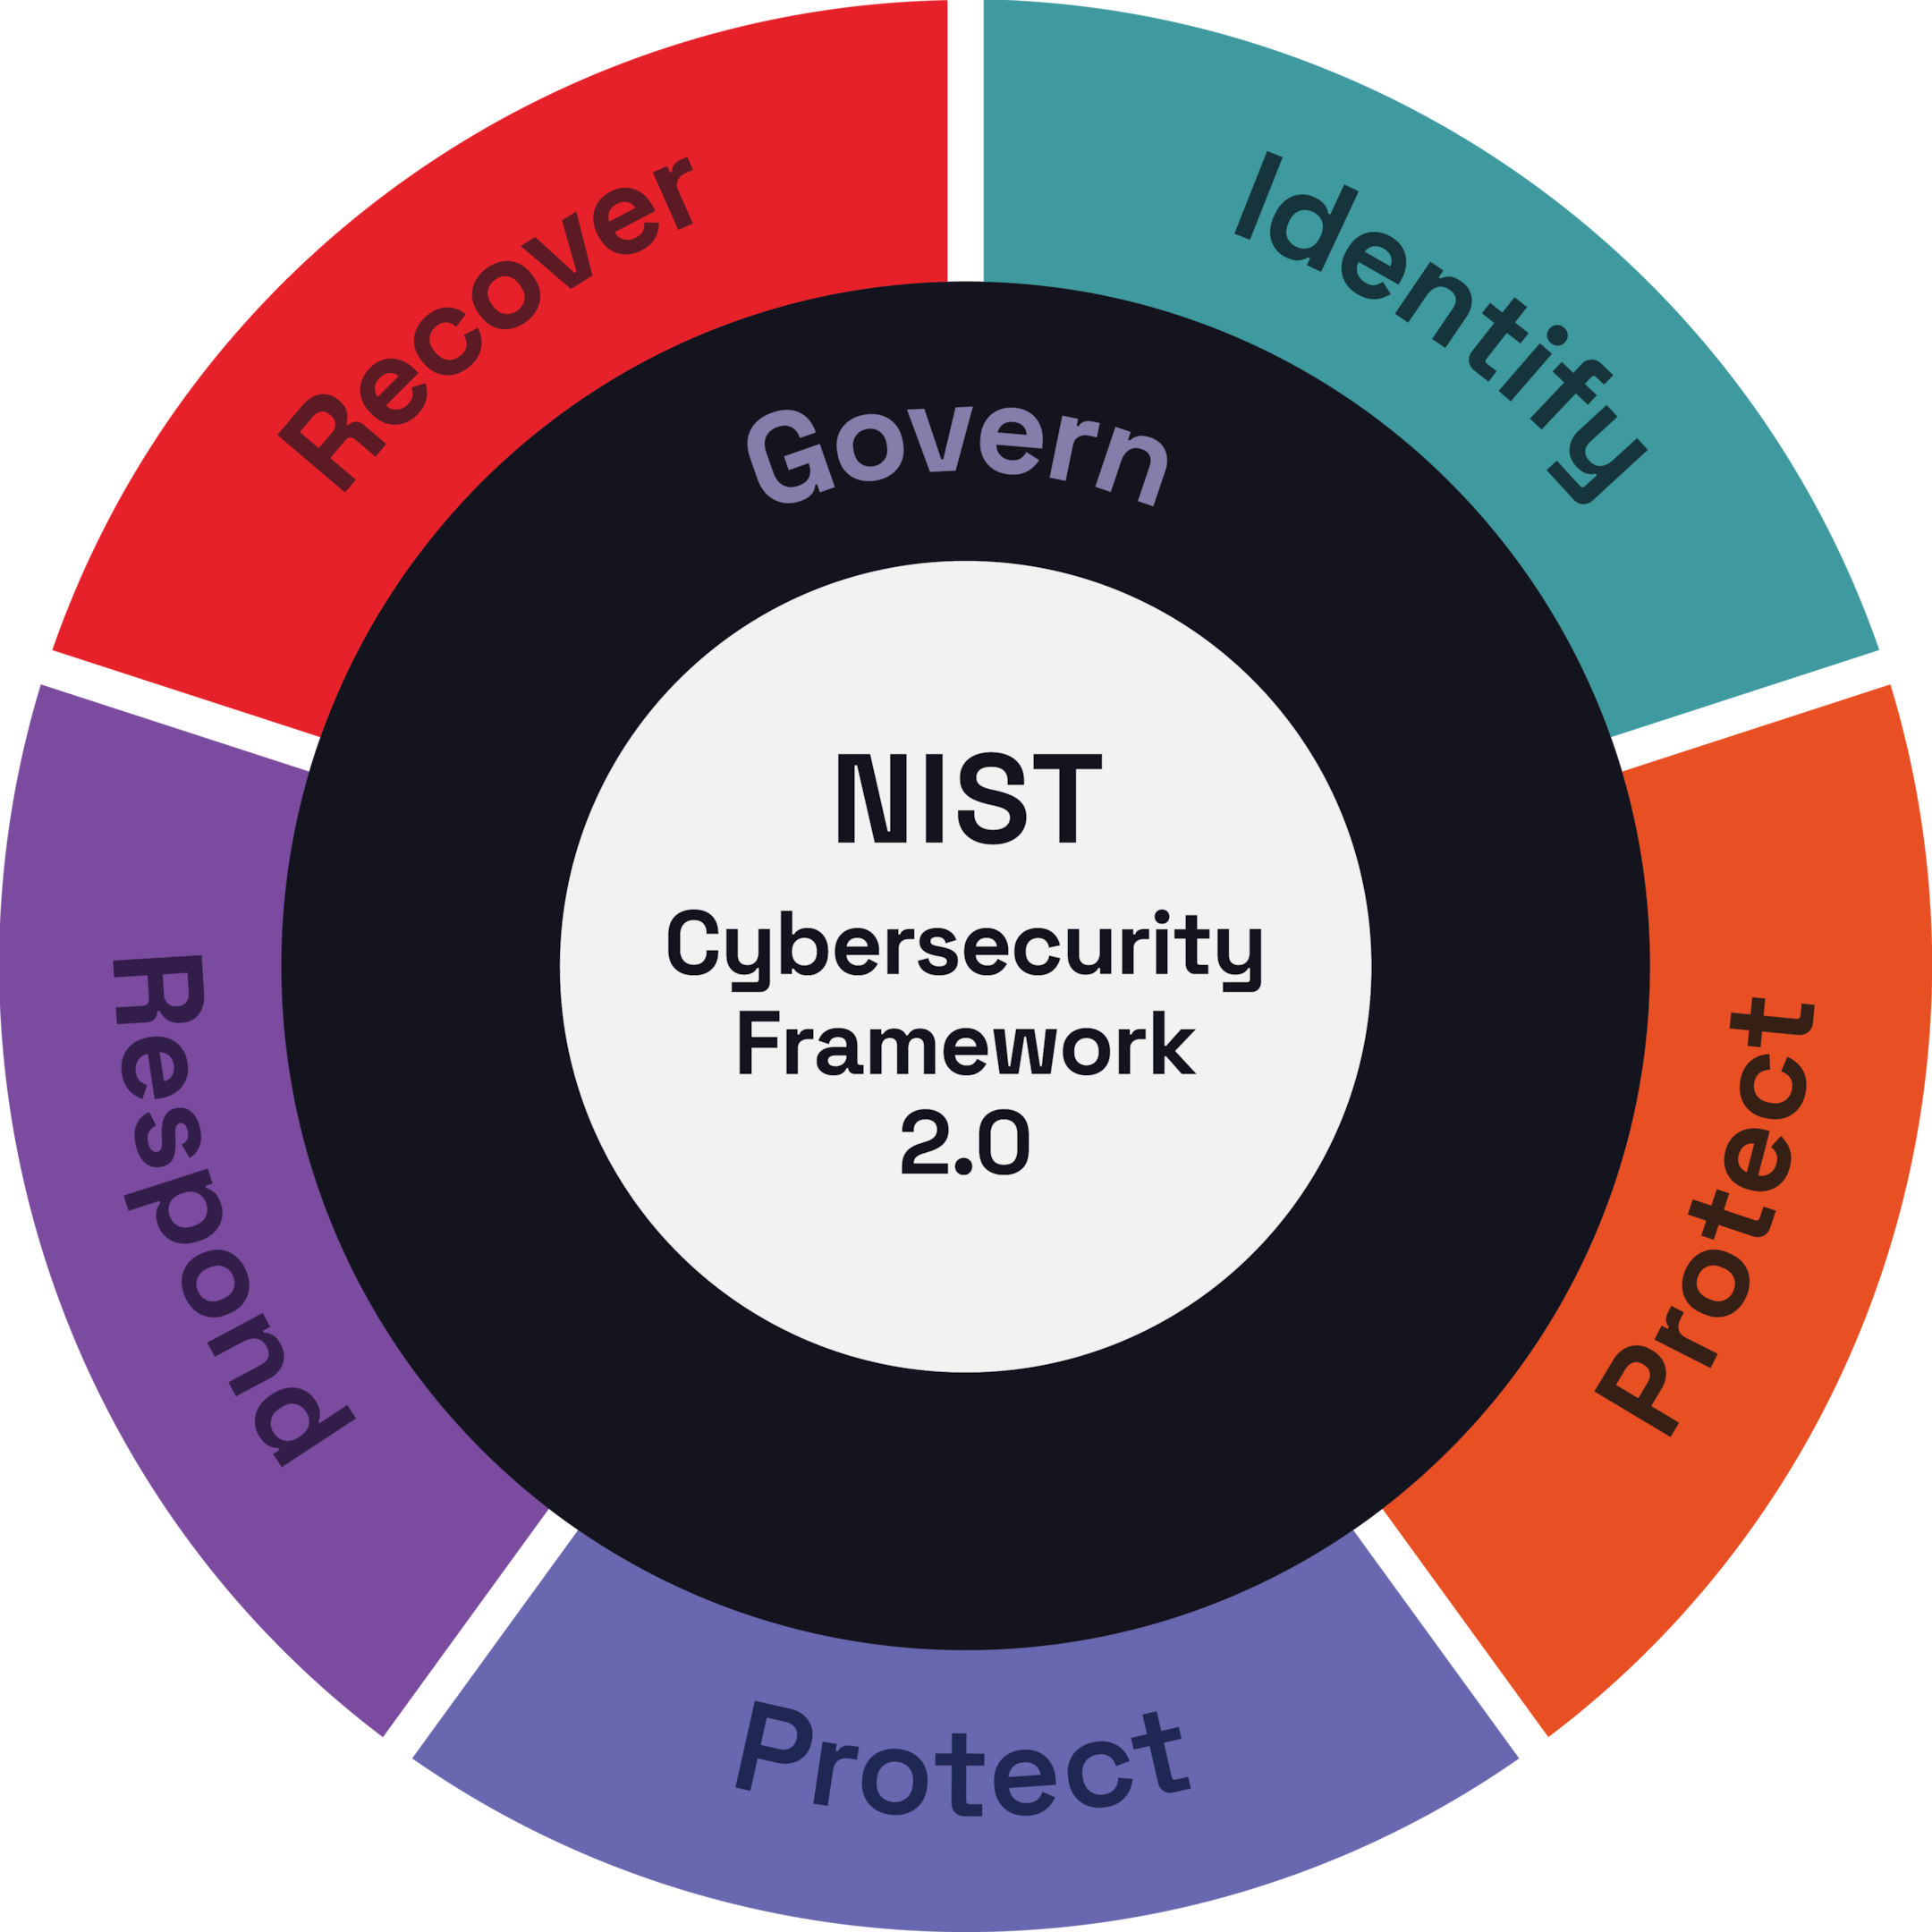
\includegraphics[width=0.8\textwidth]{img/NIST-cyber-security-framework2.0.png}
\caption{NIST Siber Güvenlik Çerçevesi 2.0 (CSF 2.0) - Altı Ana İşlev}
\label{fig:nist-csf}
\end{figure}

\textbf{ISO 27001 vs. NIST CSF Karşılaştırması}

ISO 27001 ve NIST CSF, bilgi güvenliği ve risk yönetimini farklı açılardan ele alan tamamlayıcı çerçevelerdir.

\begin{adjustbox}{max width=\textwidth}
\begin{tabularx}{\textwidth}{|l|X|X|}
\hline
\textbf{Özellik} & \textbf{ISO 27001} & \textbf{NIST CSF} \\
\hline
\textbf{Yapısı} & Bir standarttır. Uygunluğu kanıtlamak için belirli ölçütleri karşılamanız gereken bir test gibidir. & Bir rehber veya kılavuzdur. Kuruluşlara siber güvenlik programı oluşturmaları için yol gösterir. \\
\hline
\textbf{Amacı} & Mevcut bir siber güvenlik programını güçlendirmek ve standardizasyon yoluyla güven oluşturmak için idealdir. & Siber güvenlik yolculuğunun erken aşamalarında olan veya yapılandırılmış bir yaklaşım arayan kuruluşlar için en iyisidir. \\
\hline
\textbf{Kapsamı} & Uluslararası kabul görmüştür. Genellikle büyük şirketler tarafından satıcılarından istenen bir gerekliliktir. & ABD federal kurumlarına yardımcı olmak için kurulmuştur, ancak herhangi bir kuruluş tarafından kullanılabilir. Müşteriler tarafından nadiren istenen bir gerekliliktir. \\
\hline
\textbf{Maliyeti} & Üçüncü taraf denetimleri ve sertifikasyon süreci nedeniyle maliyetlidir (5.000 ila 15.000 ABD Doları veya daha fazla). & Ücretsiz erişilebilir. Üçüncü taraf denetimi veya sertifikasyon gerektirmez. \\
\hline
\textbf{Sertifikasyon} & Resmi bir denetim süreci ve sertifika gerektirir. & Resmi bir sertifika süreci yoktur. Kuruluşlar uyumluluğu kendileri rapor edebilir. \\
\hline
\end{tabularx}
\end{adjustbox}

Her iki çerçeve de benzer risk yönetimi süreçlerine dayanır ve önemli ölçüde örtüşür. Bir kuruluşa göre, NIST CSF uygulayan bir şirket, ISO 27001 uyumluluğuna \%80 oranında yaklaşmış olur ve ISO 27001 de NIST CSF yönergelerinin yarısından fazlasını içerir.

\subsection{COBIT 5 IT Governance Framework}

COBIT (Control Objectives for Information and Related Technology), Bilgi Sistemleri Denetim ve Kontrol Birliği (ISACA) tarafından geliştirilen ve BT'nin iş hedefleriyle hizalanmasını sağlamak için kullanılan bir yönetişim çerçevesidir. COBIT 5, BT'nin kurumsal hedeflere değer katmasını sağlamak için beş temel prensibe dayanır:

\begin{enumerate}
    \item \textbf{Paydaş İhtiyaçlarını Karşılama:} Çerçeve, BT'nin tüm paydaşların ihtiyaçlarını karşılayacak şekilde değer yaratmasına odaklanır.
    \item \textbf{Kuruluşu Baştan Sona Kapsama:} COBIT 5, BT yönetişimini kuruluşun tüm süreçlerine, departmanlarına ve işlevlerine entegre etmeyi hedefler.
    \item \textbf{Tek Bir Entegre Çerçeve Uygulama:} COBIT 5, diğer en iyi uygulama çerçeveleri ve standartlarla (ITIL, ISO 20000, ISO 27001 gibi) entegre çalışacak şekilde tasarlanmıştır. Bu, kuruluşların tek bir çerçeveye bağlı kalmak yerine, ihtiyaçlarına göre farklı standartların en iyi yönlerini birleştiren hibrit bir yaklaşım benimsemesini sağlar.
    \item \textbf{Bütünsel Bir Yaklaşımı Etkinleştirme:} Bu ilke, BT yönetişiminin başarıya ulaşması için sadece süreçlere değil, aynı zamanda organizasyonel yapılara, kültüre, bilgiye, hizmetlere ve insan kaynaklarına da odaklanılması gerektiğini vurgular.
    \item \textbf{Yönetişimi Yönetimden Ayırma:} COBIT, "yönetişim" (governance) ve "yönetim" (management) kavramlarını net bir şekilde ayırır. Yönetişim, paydaşların ihtiyaçlarını değerlendirme, yönlendirme ve performansı izleme ile ilgilenirken; yönetim, planlama, inşa etme, çalıştırma ve izleme ile ilgilenir.
\end{enumerate}

Bu prensipler, bir kuruluşun BT yatırımlarından beklenen değeri gerçekleştirmesine yardımcı olur. COBIT'in diğer framework'lerle entegre bir şekilde çalışmak üzere tasarlanmış olması, modern BT yönetişiminin çok boyutlu ve karmaşık doğasını yansıtan bir yaklaşımdır.

\subsection{COSO Internal Control Framework}

COSO (Committee of Sponsoring Organizations of the Treadway Commission), bir kuruluşun iç kontrol süreçlerini tasarlamasına ve uygulamasına yardımcı olan bir çerçevedir. COSO'ya göre, iç kontrol, operasyonel, finansal raporlama ve uyumluluk hedeflerine ulaşma konusunda makul bir güvence sağlamak için tasarlanmış bir süreçtir. Çerçeve, beş ana bileşenden oluşur:

\begin{enumerate}
    \item \textbf{Kontrol Ortamı (Control Environment):} Bir kuruluşun etik değerlere, dürüstlüğe ve liderlik taahhüdüne olan bağlılığını gösterir.
    \item \textbf{Risk Değerlendirmesi (Risk Assessment):} Kuruluşun hedeflerine ulaşmasını etkileyebilecek riskleri tanımlama ve analiz etme sürecidir.
    \item \textbf{Kontrol Faaliyetleri (Control Activities):} Riskleri azaltmak için tasarlanmış politikalar ve prosedürlerdir. Örneğin, erişim kontrolleri ve güvenlik politikaları bu kapsamdadır.
    \item \textbf{Bilgi ve İletişim (Information and Communication):} İç ve dış iletişim kanallarının yasal, etik ve sektörel standartlara uygun olmasını sağlar. Bu, doğru bilginin zamanında ilgili taraflara iletilmesini içerir.
    \item \textbf{İzleme (Monitoring):} Kontrollerin etkinliğinin sürekli olarak değerlendirilmesi ve gözden geçirilmesidir. Bu, dahili ve harici denetimlerle gerçekleştirilebilir.
\end{enumerate}

COSO, kuruluşların iç kontrollerini iş süreçlerine entegre etmelerini sağlayarak, yasal ve düzenleyici gerekliliklere uyumlarını kolaylaştırır.

\subsection{PCI DSS Payment Card Industry Standards}

PCI DSS (Payment Card Industry Data Security Standard), ödeme kartı verilerini (örneğin, kredi kartı bilgileri) işleyen, saklayan veya ileten tüm kuruluşlar için geçerli olan bir güvenlik standartları setidir.



\subsection{HITRUST Ortak Güvenlik Çerçevesi (CSF)}

\begin{figure}[H]
    \centering
    
\includegraphics[width=0.6\textwidth]{img/HITRUSTCSFCertifiedLogo.png}
    \caption{HITRUST CSF (Common Security Framework) Sertifikası}
    \label{fig:hitrust-csf}
\end{figure}

HITRUST CSF (Common Security Framework), özellikle sağlık sektörü için tasarlanmış kapsamlı bir güvenlik ve gizlilik çerçevesidir. Bu çerçeve, HIPAA, GDPR, ISO, NIST gibi birçok farklı standardı ve düzenlemeyi tek bir çatı altında birleştirir.

\begin{itemize}
\item \textbf{Yapı ve Bileşenler:}
\begin{itemize}
    \item 14 güvenlik kategorisi
    \item 49 kontrol alanı
    \item 156 kontrol referansı
    \item 3 olgunluk seviyesi
\end{itemize}

\item \textbf{Olgunluk Modeli:} HITRUST CSF, her kontrolün olgunluğunu 5 seviyede değerlendirir:
\begin{enumerate}
    \item Politika
    \item Prosedürler
    \item Uygulama
    \item Ölçüm
    \item Yönetim
\end{enumerate}

\item \textbf{Sertifikasyon Süreci:}
\begin{itemize}
    \item Öz-değerlendirme
    \item Doğrulanmış değerlendirme
    \item Sertifikalı değerlendirme
\end{itemize}

\item \textbf{Faydaları:}
\begin{itemize}
    \item Birden fazla düzenleme ve standardın tek bir çerçevede birleştirilmesi
    \item Risk bazlı yaklaşım
    \item Ölçeklenebilir ve özelleştirilebilir kontroller
    \item Sürekli iyileştirme modeli
\end{itemize}
\end{itemize} Standardın temel amacı, kart verilerini koruyarak dolandırıcılığı önlemektir. PCI DSS, 12 ana gereksinimden oluşur. Bu gereksinimlerden biri, kullanıcı kimliklendirmesi ve erişim kontrolü ile ilgilidir.

\textbf{Temel Gereksinimler ve Uygulama}

\begin{itemize}
    \item \textbf{Gereksinim 8: Kullanıcı Kimliklendirmesi:} Bu gereksinim, bilgisayara erişimi olan her bir kişiye benzersiz bir tanıtıcı atamasını zorunlu kılar. Ayrıca, güçlü parola politikaları gerektirir:
    \begin{itemize}
        \item Parolalar en az 90 günde bir değiştirilmelidir.
        \item Parola uzunluğu en az 7 karakter olmalıdır.
        \item Parolalar hem sayısal hem de alfabetik karakterler içermelidir.
        \item Kullanıcıların önceki dört parolasıyla aynı yeni bir parola belirlemesi engellenmelidir.
    \end{itemize}
    \item \textbf{Kapsam Belirleme:} PCI DSS uyumluluğu için, öncelikle kart verilerinin işlendiği, saklandığı veya iletildiği tüm sistemleri ve uygulamaları içeren Kart Sahibi Veri Ortamının (Card Holder Data Environment - CDE) doğru bir şekilde belirlenmesi gerekir. Bu, gereksinimlerin hangi sistemlere uygulanacağını netleştirir.
\end{itemize}

PCI DSS, kuruluşların kart verilerini korumak için teknik ve yönetsel kontrolleri uygulamalarını zorunlu kılar.

\section{Veri Sınıflandırması ve Yaşam Döngüsü Yönetimi}

Veri sınıflandırması ve yaşam döngüsü yönetimi, verilerin doğru şekilde korunmasını, yönetilmesini ve nihayetinde güvenli bir şekilde imha edilmesini sağlamak için kritik öneme sahip süreçlerdir. Bu süreçler, kuruluşların yasal düzenlemelere (örneğin GDPR veya KVKK) uymasına ve veri kaybı riskini azaltmasına yardımcı olur.

\subsection{Veri Kategorileri: Public, Internal, Confidential, Restricted}

Veri sınıflandırması, verileri hassasiyetine ve önemine göre kategorize ederek her kategoriye uygun güvenlik önlemlerinin uygulanmasını sağlar. Tipik olarak, veriler dört ana kategoriye ayrılır:

\begin{itemize}
    \item \textbf{Public (Genel):} Bu veriler, herhangi bir kısıtlama olmaksızın serbestçe kullanılabilir, yeniden kullanılabilir ve yeniden dağıtılabilir. Örnekler arasında basın bültenleri, şirket tanıtım materyalleri ve iş tanımları yer alır.
    \item \textbf{Internal (Kurum İçi):} Bu veriler yalnızca şirket personeli veya erişim yetkisi verilen çalışanlar için tasarlanmıştır. Yetkisiz ifşası genellikle büyük bir zarara yol açmaz, ancak yine de gizli tutulmalıdır. İç yazışmalar veya iş planları bu kategoriye örnek verilebilir.
    \item \textbf{Confidential (Gizli):} Gizli veriler, yetkili erişim ve özel yetkilendirme gerektirir. Bu verilerin yetkisiz ifşası veya kötüye kullanımı, şirkete önemli zararlar verebilir. Sosyal güvenlik numaraları (SSN) veya kart sahibi verileri (Cardholder Data) bu kategoride yer alır. Bu veriler, genellikle HIPAA veya PCI DSS gibi yasalarla korunur.
    \item \textbf{Restricted (Kısıtlı):} Bu, en yüksek hassasiyet seviyesine sahip veri kategorisidir. Kısıtlı verilerin yetkisiz erişimi veya ifşası, yasal suçlamalara, çok yüksek para cezalarına ve geri dönülemez itibar kaybına yol açabilir. Şirketin mülkiyetinde olan araştırma ve geliştirme verileri veya federal düzenlemelerle korunan veriler bu kategoriye girer.
\end{itemize}

\subsection{Data Ownership ve Data Stewardship Modelleri}

Veri sahipliği (Data Ownership) ve veri sorumluluğu (Data Stewardship), veri yönetişiminde iki farklı ancak birbirini tamamlayan roldür.

\begin{itemize}
    \item \textbf{Veri Sahibi (Data Owner):} Bir veri kümesi üzerinde nihai karar verme yetkisine ve hesap verebilirliğe sahip olan kişidir. Veri sahipleri, verinin nasıl kullanılacağına, erişileceğine ve saklanacağına dair politikaları ve stratejik yönü tanımlarlar. Örneğin, bir finans departmanının verilerinin sahibi genellikle CFO'dur.
    \item \textbf{Veri Sorumlusu (Data Steward):} Veri sahibinin belirlediği politikaları operasyonel düzeyde uygulayan ve günlük veri yönetimi faaliyetlerini yürüten kişidir. Veri sorumluları, veri kalitesini, tutarlılığını ve uyumluluğunu sağlamaktan sorumludur.
\end{itemize}

Aşağıdaki tablo, bu iki rol arasındaki temel farkları özetlemektedir:

\begin{tabular}{|p{3cm}|p{6.5cm}|p{6cm}|}
\hline
\textbf{Özellik} & \textbf{Veri Sahibi (Data Owner)} & \textbf{Veri Sorumlusu (Data Steward)} \\
\hline
\textbf{Yetki} & Veri kullanımı, erişimi ve saklanması hakkında nihai kararları verme yetkisi vardır. & Veri sahibinin belirlediği politikaları uygular ve operasyonel yönetimi yürütür. \\
\hline
\textbf{Odak Alanı} & Stratejik yön, risk yönetimi ve politika tanımına odaklanır. & Günlük veri kalitesini, tutarlılığını ve uyumluluğunu sağlamaya odaklanır. \\
\hline
\textbf{Sorumluluk} & Veri güvenliği politikalarını tanımlamak, riskleri yönetmek ve uyumluluğu sağlamaktan doğrudan sorumludur. & Veri kalitesini güvence altına almak, veriyi sınıflandırmak, dokümantasyon sağlamak ve uyumluluk kontrollerine yardımcı olmaktan sorumludur. \\
\hline
\end{tabular}

Veri sahipleri ve veri sorumluları, etkili bir veri yönetimi stratejisi için yakın iş birliği içinde çalışmalıdır.

\subsection{Veri Yaşam Döngüsü Yönetimi}

Veri yaşam döngüsü (Data Lifecycle), bir verinin ilk oluşturulduğu andan nihai olarak imha edildiği ana kadar geçtiği aşamalar dizisini ifade eder. Bu döngünün etkili bir şekilde yönetilmesi, verilerin güvenli, düzenlemelere uygun ve karar alma için erişilebilir kalmasını sağlar.

\textbf{Veri Yaşam Döngüsü Aşamaları:}

\begin{itemize}
    \item \textbf{Yaratma veya Edinme (Creation/Acquisition):} Veri yaşam döngüsü, verilerin müşteri etkileşimleri, işlemler, IoT cihazları veya manuel girişler gibi çeşitli kaynaklar aracılığıyla üretilmesiyle başlar. Bu aşamada, toplanan verilerin kalitesi ve alakalılığı sonraki tüm aşamalar için temel oluşturur.
    \item \textbf{Depolama (Storage):} Veriler yaratıldıktan sonra, veritabanları, veri gölleri veya bulut depolama gibi ortamlarda saklanır. Hassas bilgileri korumak ve yetkili kullanıcıların erişimini kolaylaştırmak için sağlam yedekleme ve kurtarma süreçlerinin uygulanması bu aşamada kritiktir.
    \item \textbf{Kullanım (Use):} Depolanan veriler, iş stratejilerini yönlendiren içgörüler elde etmek için analiz edilir. Veri analitiği araçları, verilerdeki kalıpları, eğilimleri ve anormallikleri ortaya çıkarmada önemli bir rol oynar. Bu aşamada, yetkisiz erişimi veya kötüye kullanımı en aza indirmek için uygun kullanım politikalarının uygulanması gerekir.
    \item \textbf{Paylaşım (Share):} Yetkili kullanıcılar veya kuruluşlar arasında veri aktarımı ve paylaşımı yapılır. Bu aşamada, gizlilik ve bütünlük ilkelerinin korunması için şifreleme ve erişim kontrolleri gibi güvenlik önlemleri uygulanmalıdır.
    \item \textbf{Arşivleme (Archive):} Veri, aktif ortamdaki kaynakları boşaltmak amacıyla daha az sıklıkta erişildiği zamanlarda güvenli, düşük maliyetli bir depolama ortamına taşınır. Bu aşama, verilerin yasal saklama süreleri dolana kadar korunmasını sağlar.
    \item \textbf{İmha (Destroy):} Döngünün son aşamasıdır ve artık gerekmeyen verilerin güvenli bir şekilde yok edilmesini içerir. Bu süreç, yasal ve düzenleyici gerekliliklere uyum sağlamak için dikkatle yönetilmelidir.
\end{itemize}

Veri yaşam döngüsü modeli, verinin durağan bir varlık olmadığını, aksine sürekli değişen bir dizi aşamadan geçtiğini gösterir. Bu, her aşama için özel güvenlik politikaları ve kontrolleri gerektirir. Örneğin, veri "kullanım" aşamasında DLP (Veri Kaybı Önleme) kontrolleri gerekirken, "imha" aşamasında güvenli silme yöntemleri (fiziksel imha, üzerine yazma) zorunlu hale gelir. Bu dinamik, statik, tek boyutlu güvenlik çözümlerinin neden yetersiz kaldığını açıklar.

\subsection{Metadata Yönetimi ve Otomatik Sınıflandırma Araçları}

Metadata, verinin içeriği hakkında bilgi sağlayan veridir (örneğin, bir dosyanın oluşturulma tarihi, sahibi veya kaynağı gibi) ve otomatik veri sınıflandırması için kritik bir unsurdur. Otomatik sınıflandırma araçları, önceden tanımlanmış kural setleri veya içerik inceleme teknikleri kullanarak belirli bir dosya veya mesajın hassasiyetini belirler ve uygun şekilde etiketler.

Otomatik sınıflandırma, ERP sistemleri tarafından üretilen raporlar gibi, kullanıcı müdahalesi olmadan oluşturulan veriler için özellikle faydalıdır. Ancak, bu araçlar her zaman verinin bağlamını anlayamayabilir ve bu da yanlış eşleşmelere veya hassas verileri kaçırmaya neden olabilir. Bu tür zorlukları aşmak için, otomasyon ile kullanıcı odaklı yaklaşımlar birleştirilebilir. Örneğin, otomatik olarak bir etiket önerisi sunularak kullanıcıdan onay istenebilir. Bu yaklaşım, sistemin doğruluğunu büyük ölçüde artırır ve kullanıcı güvenini sağlar.

Otomatik sınıflandırma araçları, DLP yazılımları ile entegre bir şekilde çalışarak, verinin hassasiyetine göre otomatik olarak kontrol edilmesini ve uygun politikanın uygulanmasını sağlar. Örneğin, "Gizli" olarak etiketlenmiş bir belgenin ağ üzerinden dışarıya aktarılması otomatik olarak engellenebilir.

\subsection{Veri Saklama ve İmha Politikaları}

Veri saklama (data retention) ve imha (disposal) politikaları, hangi verilerin ne kadar süreyle saklanacağını ve artık gerek duyulmayan verilerin nasıl güvenli bir şekilde yok edileceğini belirleyen yazılı kurallar bütünüdür. Bu politikalar, yasal ve düzenleyici gerekliliklere uyum sağlamak, depolama maliyetlerini azaltmak ve şirketi potansiyel davalardan korumak için hayati öneme sahiptir.

Veri imha yöntemleri, verilerin hassasiyetine ve ilgili mevzuat gerekliliklerine bağlı olarak seçilmelidir. Başlıca imha yöntemleri şunlardır:

\begin{enumerate}
    \item \textbf{Mantıksal Silme:} Bu yöntemler, veriyi geri getirilemez hale getirmek için yazılımsal teknikler kullanır.
    \begin{itemize}
        \item \textbf{Temizleme (Clearing):} Veri depolama cihazlarının üzerine yeni veriler yazılarak eski verilerin kurtarılmasını zorlaştıran bir tekniktir. Bu, orta düzeyde bir güvenlik sağlar.
        \item \textbf{Arındırma (Purging):} Fiziksel teknikler veya ileri teknoloji kullanarak verileri okunamaz ve laboratuvar ortamında bile kurtarılamaz hale getiren bir yöntemdir. Degaussing veya kriptografik parçalama gibi teknikler bu amaçla kullanılır.
    \end{itemize}
    \item \textbf{Fiziksel Yok Etme:} Bu yöntem, depolama ortamını tamamen yok ederek verilerin geri getirilemez hale gelmesini sağlar. Bu, hassas veriler için en yüksek güvenlik seviyesini sunar. Örnekler arasında optik veya manyetik medyanın eritilmesi, yakılması, toz haline getirilmesi veya parçalanması yer alır.
\end{enumerate}

Aşağıdaki tablo, veri imha yöntemlerini ve güvenlik seviyelerini karşılaştırmaktadır:

\begin{tabular}{|p{3.5cm}|p{5cm}|p{2.8cm}|p{4.2cm}|}
\hline
\textbf{Yöntem} & \textbf{Tanım} & \textbf{Güvenlik Seviyesi} & \textbf{Kullanım Alanı} \\
\hline
\textbf{Clearing (Temizleme)} & Verilerin üzerine yeni veriler yazılarak kurtarılmasının zorlaştırılması. & Orta & Daha az hassas veriler veya dahili kullanım için. \\
\hline
\textbf{Purging (Arındırma)} & Fiziksel teknikler veya özel algoritmalarla verilerin kurtarılamaz hale getirilmesi. & Yüksek & Hassas veriler veya regülasyonlara tabi veriler için. \\
\hline
\textbf{Physical Destruction} & Depolama cihazının eritme, yakma, parçalama gibi yöntemlerle fiziksel olarak yok edilmesi. & En Yüksek & En hassas ve yasal yükümlülük taşıyan veriler için. \\
\hline
\end{tabular}

Bu politikalar, depolama alanını boşaltmanın yanı sıra, gelecekteki operasyonlar için hayati varlıkların yanlışlıkla silinmesini de önler.

\section{Şifreleme Teknolojileri ve Anahtar Yönetimi}

Şifreleme, verileri okunamaz bir biçime dönüştürerek yetkisiz erişimi engelleyen temel bir bilgi güvenliği teknolojisidir. Bu teknolojinin doğru şekilde kullanılması, verilerin hem durağan (at rest) hem de hareket halindeyken (in transit) korunmasını sağlar.

\subsection{Simetrik ve Asimetrik Şifreleme Algoritmaları (AES, RSA, ECC)}

Şifreleme algoritmaları iki ana kategoriye ayrılır:

\begin{itemize}
    \item \textbf{Simetrik Şifreleme:} Bu yöntemde, hem şifreleme hem de şifre çözme için tek ve aynı gizli anahtar kullanılır. Yüksek performans sunduğu için büyük veri setlerinin şifrelenmesinde idealdir. \textbf{AES (Advanced Encryption Standard)}, günümüzde en yaygın kullanılan simetrik algoritmadır. Çeşitli anahtar uzunlukları (128, 192, 256 bit) sunar ve kablosuz ağ güvenliği, SSL/TLS protokolleri ve VPN'ler gibi birçok alanda kullanılır.
    \item \textbf{Asimetrik Şifreleme:} Bu yöntem, \textbf{açık anahtar} (public key) ve \textbf{özel anahtar} (private key) olmak üzere, matematiksel olarak ilişkili iki farklı anahtar kullanır. Açık anahtar herkesle paylaşılabilirken, özel anahtar yalnızca sahibinde gizli kalır. Veri açık anahtarla şifrelenir ve yalnızca ilgili özel anahtarla çözülebilir. Simetrik şifrelemeye göre daha yavaştır, bu nedenle genellikle küçük veri setlerinin (oturum anahtarları gibi) şifrelenmesi ve dijital imzalar için kullanılır.
\end{itemize}

Asimetrik şifrelemede kullanılan ana algoritmalar şunlardır:

\begin{itemize}
    \item \textbf{RSA (Rivest–Shamir–Adleman):} Güvenliği, büyük sayıları çarpanlarına ayırmanın zorluğuna dayanır. Yaygın olarak kullanılan bir algoritmadır, ancak modern tehditlere karşı daha uzun anahtar boyutları (örneğin, 2048 veya 3072 bit) gerektirebilir.
    \item \textbf{ECC (Elliptic Curve Cryptography):} RSA'ya göre daha modern ve verimli bir alternatiftir. Aynı kriptografik gücü, çok daha küçük anahtar boyutlarıyla sağlar. Bu, mobil cihazlar ve Nesnelerin İnterneti (IoT) gibi sınırlı işlem gücüne sahip ortamlar için idealdir.
\end{itemize}

Aşağıdaki tablo, bu algoritmaların teknik özelliklerini özetlemektedir:

\begin{tabular}{|p{3.5cm}|p{4cm}|p{4cm}|p{4cm}|}
\hline
\textbf{Özellik} & \textbf{Simetrik (AES)} & \textbf{Asimetrik (RSA)} & \textbf{Asimetrik (ECC)} \\
\hline
\textbf{Anahtar Sayısı} & 1 (Gizli anahtar) & 2 (Açık ve özel anahtar) & 2 (Açık ve özel anahtar) \\
\hline
\textbf{Anahtar Boyutu} & 128, 192, 256 bit & 2048, 3072, 7680 bit & 224, 256, 384 bit \\
\hline
\textbf{Performans} & Çok Hızlı & Yavaş & Daha Hızlı \\
\hline
\textbf{Temel Fonksiyon} & Toplu veri şifreleme & Dijital imza, anahtar değişimi & Dijital imza, anahtar değişimi \\
\hline
\end{tabular}

\textbf{Adım Adım Kod Örnekleri (Python)}

\textbf{Simetrik Şifreleme (AES) Örneği:}

\texttt{cryptography} kütüphanesi ile AES-GCM modunda şifreleme.

\begin{verbatim}
from cryptography.hazmat.primitives.ciphers.aead import AESGCM
import os
 
# Rastgele 256-bit anahtar ve nonce oluştur
key = os.urandom(32)
nonce = os.urandom(12)
 
# Şifrelenecek metin
plaintext = b"Gizli mesajimiz."
 
# Şifreleme işlemi
aesgcm = AESGCM(key)
ciphertext = aesgcm.encrypt(nonce, plaintext, None)
 
print(f"Şifrelenmiş metin: {ciphertext.hex()}")
 
# Şifre çözme işlemi
try:
    decrypted_text = aesgcm.decrypt(nonce, ciphertext, None)
    print(f"Şifresi çözülmüş metin: {decrypted_text.decode('utf-8')}")
except Exception as e:
    print(f"Hata: {e}")
\end{verbatim}

\textbf{Asimetrik Şifreleme (RSA) Örneği:}

\texttt{cryptography} kütüphanesi ile RSA anahtar çifti oluşturma ve şifreleme.

\begin{verbatim}
from cryptography.hazmat.primitives.asymmetric import rsa
from cryptography.hazmat.primitives import serialization
from cryptography.hazmat.primitives.asymmetric import padding
from cryptography.hazmat.primitives import hashes
 
# Özel anahtar oluşturma
private_key = rsa.generate_private_key(
    public_exponent=65537,
    key_size=2048,
)
 
# Açık anahtarı türetme
public_key = private_key.public_key()
 
# Şifrelenecek veri
message = b"Bu mesaj RSA ile sifrelenecek."
 
# Açık anahtar ile veriyi şifreleme
encrypted = public_key.encrypt(
    message,
    padding.OAEP(
        mgf=padding.MGF1(algorithm=hashes.SHA256()),
        algorithm=hashes.SHA256(),
        label=None
    )
)
 
print(f"Şifrelenmiş veri: {encrypted.hex()}")
 
# Özel anahtar ile şifre çözme
decrypted = private_key.decrypt(
    encrypted,
    padding.OAEP(
        mgf=padding.MGF1(algorithm=hashes.SHA256()),
        algorithm=hashes.SHA256(),
        label=None
    )
)
 
print(f"Şifresi çözülmüş veri: {decrypted.decode('utf-8')}")
\end{verbatim}

\subsection{Hash Fonksiyonları ve Dijital İmzalar}

Hash fonksiyonları, verinin bütünlüğünü sağlamak için kullanılan tek yönlü matematiksel algoritmalardır. Bir girdi (mesaj) ne kadar büyük olursa olsun, sabit boyutlu bir çıktı (özet veya hash değeri) üretir. Bu çıktının en önemli özelliği, girdideki en ufak bir değişikliğin bile çıktıda tamamen farklı bir değere neden olmasıdır ("çığ etkisi"). Bu tek yönlü özellik, özet değerinden orijinal verinin elde edilememesini sağlar.

Hash fonksiyonları, \textbf{dijital imza} sürecinde kritik bir rol oynar. Dijital imza, bir belgenin bütünlüğünü ve kaynağını doğrulamak için kullanılır. Eğer belgenin kendisi çok büyükse, tüm belgeyi imzalamak zaman alıcı ve kaynak yoğundur. Bunun yerine, belgenin hash değeri alınır ve bu küçük boyutlu özet değeri, göndericinin özel anahtarıyla imzalanır. Alıcı, imzalı özet değerini göndericinin açık anahtarıyla doğrulayarak mesajın bütünlüğünü kontrol eder. Bu yöntem, hem operasyonel maliyeti hem de iletişim yükünü önemli ölçüde azaltır.

\subsection{Açık Anahtar Altyapısı (PKI) ve Sertifika Yönetimi}

Açık Anahtar Altyapısı (PKI), dijital sertifikaları ve anahtar çiftlerini oluşturmak, yönetmek, dağıtmak, saklamak ve iptal etmek için gerekli olan bir dizi rol, politika, donanım, yazılım ve prosedürdür. PKI'nın temel amacı, elektronik iletişimin güvenli bir şekilde aktarılmasını sağlamak, tarafların kimliğini doğrulamak ve verinin bütünlüğünü güvence altına almaktır.

PKI'nın temel bileşenleri şunlardır:

\begin{itemize}
    \item \textbf{Sertifika Otoritesi (CA - Certificate Authority):} Güvenilir bir üçüncü taraf olan CA, dijital sertifikaları düzenler, imzalar ve iptal eder. Bir CA, kendi özel anahtarını kullanarak sertifikaları dijital olarak imzalar, böylece son kullanıcı sertifikasına olan güven, CA'nın anahtarına olan güvene dayanır.
    \item \textbf{Kayıt Otoritesi (RA - Registration Authority):} RA, bir sertifika talebinde bulunan kişinin kimliğini doğrulayan bir bileşendir. RA, talepleri alır, gerekli doğrulamaları yapar ve ardından sertifikanın düzenlenmesi için talebi CA'ya iletir. Güvenlik ve erişilebilirlik nedenleriyle RA genellikle CA'dan ayrı bir birim olarak işlev görür.
    \item \textbf{Sertifika Veritabanı:} Düzenlenen ve iptal edilen tüm sertifikaların saklandığı bir depodur.
    \item \textbf{Güven Zinciri (Chain of Trust):} Bu, bir Kök CA'dan başlayıp, ara CA'lar aracılığıyla son kullanıcı sertifikalarına kadar uzanan hiyerarşik bir yapıdır. Bir sertifikanın doğruluğu, zincirdeki her bir sertifikanın bir üst otorite tarafından imzalanmış olmasıyla doğrulanır. Bu zincir, bir sertifikanın geçerliliğini kontrol etmek için kritik bir rol oynar.
\end{itemize}

\subsection{Donanım Güvenlik Modülleri (HSM) ve Anahtar Yönetim Sistemleri (KMS)}

Anahtar yönetimi, şifreleme teknolojilerinin güvenli bir şekilde uygulanabilmesi için hayati önem taşır. Bu alanda iki temel teknoloji öne çıkar: Donanım Güvenlik Modülleri (HSM) ve Anahtar Yönetim Sistemleri (KMS).

\begin{itemize}
    \item \textbf{Donanım Güvenlik Modülü (HSM):} Bir HSM, şifreleme anahtarlarını fiziksel olarak koruyan, kurcalamaya dayanıklı bir donanım cihazıdır. Bir "banka kasası"na benzetilebilir; anahtarlar HSM içinde oluşturulur, depolanır ve imha edilir ve bu cihazdan asla çıkarılamaz. FIPS 140-2 Seviye 3 gibi düzenleyici standartlara uygun olan HSM'ler, fiziksel bir saldırı durumunda anahtarları otomatik olarak yok etme yeteneğine sahiptir. Bu özelliği, onları bir "Güvenin Kökü" (Root of Trust) olarak işlev görmesi gereken kritik altyapılarda vazgeçilmez kılar.
    \item \textbf{Anahtar Yönetim Sistemi (KMS):} KMS, şifreleme anahtarlarının yaşam döngüsünü (oluşturma, rotasyon, dağıtım, depolama ve imha) büyük ölçekte yönetmeye odaklanan bir yazılım çözümüdür. KMS, erişim politikalarını uygulamayı, kullanımı izlemeyi ve denetim kayıtları tutmayı kolaylaştırır.
\end{itemize}

Sadece birini kullanmak, güvenlikte önemli boşluklar yaratabilir. Sadece KMS kullanmak "uygun ama riskli" olabilir, çünkü anahtarlar yazılımda depolandığından yanlış bir yapılandırma veya bir zafiyet nedeniyle ifşa olma riski taşır. Sadece HSM kullanmak ise "güvenli ama yönetimi zor"dur, çünkü geniş ölçekte politika uygulamayı ve anahtar rotasyonunu manuel hale getirir. Optimal çözüm, her iki teknolojinin birlikte kullanıldığı hibrit bir modeldir. Bu modelde, KMS yönetim ve ölçeklenebilirlik sağlar, HSM ise anahtarlar için en yüksek düzeyde fiziksel korumayı sunar.

\begin{adjustbox}{max width=\textwidth}
\begin{tabularx}{\textwidth}{|l|X|X|X|}
\hline
\textbf{Özellik} & \textbf{Sadece HSM} & \textbf{Sadece KMS} & \textbf{KMS + HSM Birlikte Kullanımı} \\
\hline
\textbf{Anahtarın Depolandığı Yer} & Fiziksel bir donanım cihazı içinde. & Genellikle yazılım veya sanal makine içinde. & Anahtarlar HSM'de güvenli bir şekilde depolanır, ancak KMS üzerinden yönetilir. \\
\hline
\textbf{Güvenlik Riski} & Fiziksel olarak güvenlidir, ancak ölçeklenebilirlik ve yönetim eksikliği riskleri barındırır. & Kullanışlıdır, ancak yanlış yapılandırma veya zafiyetler anahtarları ifşa edebilir. & Anahtarlar güvende kalır ve kolayca yönetilebilir. \\
\hline
\textbf{Kontrol \& Yönetim} & Manuel operasyonlar gerektirir; politika uygulaması ve izleme zordur. & Kuralları belirlemek, anahtarları döndürmek ve kullanımı günlüğe kaydetmek kolaydır. & Politikaları belirlemek, izlemek ve otomatikleştirmek için güçlü bir koruma katmanı mevcuttur. \\
\hline
\textbf{Uyum Hazırlığı} & Yeterli değildir; politika kontrolü ve denetlenebilirlik eksiktir. & Yetersizdir; "güvenin kökü" eksiktir. & Entegre politika kontrolü ve donanım koruması sayesinde tam uyumluluk sağlar. \\
\hline
\end{tabularx}
\end{adjustbox}

Bu yaklaşım, siber güvenlikte "tek bir çözüm her derde deva olmaz" prensibinin bir kanıtıdır. En yüksek güvenliğin, farklı teknolojilerin en iyi yönlerini birleştiren katmanlı ve entegre çözümlerle elde edildiğini gösterir.

\subsection{Kuantum-Güvenli Kriptografi ve Post-Kuantum Algoritmaları}

Kuantum bilgisayarlar, mevcut şifreleme yöntemlerinin güvenliğini tehdit eden yeni bir risk alanıdır. Shor's algoritması gibi kuantum algoritmaları, günümüzün yaygın asimetrik şifreleme algoritmalarının (örneğin RSA) dayandığı matematiksel problemleri (büyük sayıları çarpanlarına ayırma) çözme potansiyeline sahiptir. Grover's algoritması ise simetrik algoritmaların (AES gibi) kaba kuvvet saldırılarına karşı direncini azaltabilir, ancak bu algoritmalara karşı korunmak genellikle anahtar boyutunu iki katına çıkarmakla mümkün olabilir.

\textbf{Kuantum-Güvenli Kriptografi (PQC)}, standart bilgisayarlarda çalışabilen ancak kuantum bilgisayarların saldırılarına karşı dirençli olan yeni algoritmaların geliştirilmesidir. Bu algoritmalar, kuantum bilgisayarların çözemeyeceği varsayılan matematiksel problemlere (örneğin, kafes tabanlı kriptografi) dayanır.

NIST, kuantum-güvenli kriptografi için yeni standartlar belirlemek amacıyla bir yarışma başlatmıştır. Bu süreç sonucunda \textbf{CRYSTALS-Kyber} (şifreleme) ve \textbf{CRYSTALS-Dilithium} (dijital imzalar) algoritmaları birincil standartlar olarak seçilmiştir. Bu algoritmalar, yüksek güvenlik sunmanın yanı sıra, dengeli anahtar boyutları ve güçlü performans özelliklerine sahiptir.

\section{Veri Kaybı Önleme (DLP) ve Veri Koruma Teknolojileri}

Veri Kaybı Önleme (DLP), hassas verilerin yetkisiz kişilere ifşasını, aktarımını veya sızdırılmasını tespit eden, önleyen ve yöneten bir dizi araç ve süreçtir. DLP çözümleri, bir kuruluşun fikri mülkiyetini, kişisel olarak tanımlanabilir bilgilerini (PII) korumasına ve dijital gizlilik yasalarına uymasına yardımcı olur.

\begin{figure}[H]
    \centering
    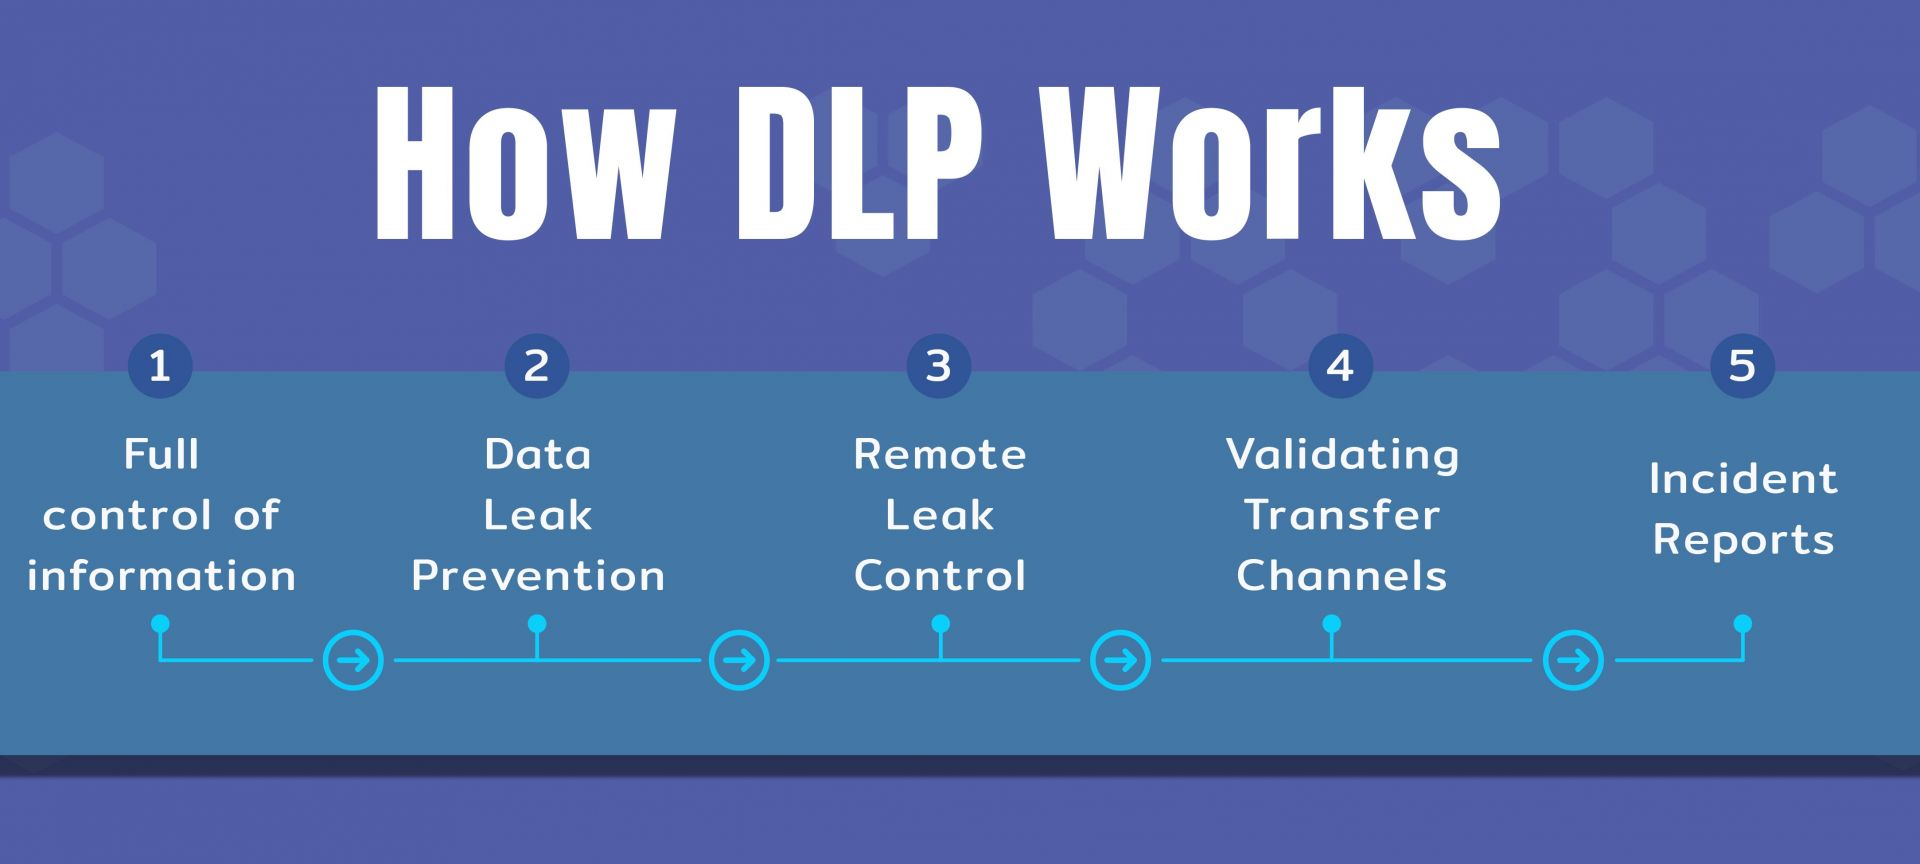
\includegraphics[width=0.8\textwidth]{img/dlp.png}
    \caption{Veri Kaybı Önleme (DLP) Teknolojileri ve Mimarisi}
    \label{fig:dlp}
\end{figure}

\subsection{Ağ Tabanlı, Uç Nokta Tabanlı ve Depolama Tabanlı DLP}

DLP çözümleri, odaklandıkları koruma alanına göre üç ana türe ayrılır:

\begin{itemize}
    \item \textbf{Ağ Tabanlı (Network-based) DLP:} Ağ trafiğini gerçek zamanlı olarak izler ve hassas verilerin e-posta veya diğer ağ protokolleri aracılığıyla yetkisiz bir şekilde dışarı aktarılmasını engeller. Geleneksel olarak, tüm çalışanların ofis ağına bağlı olduğu ve trafiğin merkezileştirildiği on-premise (yerinde) ortamlarda temel bir bileşendi. Ancak, uzaktan çalışma ve bulut tabanlı mimarilerin yaygınlaşmasıyla, ağ tabanlı DLP'nin etkinliği azalmıştır, çünkü ağın dışındaki etkinlikleri veya bulut uygulamaları arasındaki veri akışını izleyemez.
    \item \textbf{Uç Nokta Tabanlı (Endpoint-based) DLP:} Dizüstü bilgisayarlar, masaüstü bilgisayarlar ve mobil cihazlar gibi bireysel uç noktalardaki verileri kontrol eder. Bu çözümler, verilerin kaynağında nasıl kopyalandığını, taşındığını, yüklendiğini veya paylaşıldığını izler ve engeller. Kullanıcı ağa bağlı olmasa bile çalışır ve bu nedenle uzaktan çalışmanın yaygın olduğu günümüz ortamında vazgeçilmez bir çözüm haline gelmiştir.
    \item \textbf{Depolama Tabanlı (Storage-based) DLP:} Veritabanları, dosya sunucuları ve bulut depoları gibi "durağan" haldeki verileri tarar. Bu çözümler, hassas verileri keşfeder, sınıflandırır ve uygun koruma önlemlerini (örneğin, şifreleme) uygular.
\end{itemize}

Uzaktan çalışmanın yaygınlaşmasıyla birlikte, veri güvenliğinin odak noktası ağ çevresinden, verinin asıl bulunduğu yer olan uç noktalara kaymıştır. Bu, güvenlik teknolojilerinin, iş yapış biçimlerindeki köklü değişikliklere nasıl yanıt verdiğinin somut bir örneğidir. Modern bir DLP stratejisi, uç nokta tabanlı çözümlerin temel bir bileşen olmasını gerektirir.

\subsection{İçerik İnceleme (Content Inspection) ve Örüntü Eşleştirme (Pattern Matching) Teknikleri}

İçerik İnceleme, DLP çözümlerinin hassas verileri tanımlamak için veri paketlerinin içeriğini analiz ettiği bir tekniktir. Bu süreç, hassasiyet belirten anahtar kelimeleri ("gizli" gibi) ve belirli yapıları arar. İçerik incelemenin temelinde yatan en güçlü tekniklerden biri de \textbf{Örüntü Eşleştirme (Pattern Matching)}'dir. Bu teknik, daha büyük bir metin içinde belirli karakter dizilerini veya kalıpları tanımlamayı içerir ve genellikle \textbf{Düzenli İfadeler (Regular Expressions - Regex)} kullanılarak uygulanır.

\textbf{Pratik Örnekler: Hassas Veri için Düzenli İfadeler (Regex)}

DLP politikaları, finansal veriler, kişisel kimlik bilgileri veya sağlık bilgileri gibi hassas verileri tespit etmek için regex desenlerini kullanır.

\begin{itemize}
    \item \textbf{Kredi Kartı Numarası Eşleştirme (MasterCard Örneği):} \\
    MasterCard numaraları genellikle 51 ile 55 arasında başlayan 16 haneli sayılardır. Metin içinde çeşitli formatlarda (boşluklu, tireli, vb.) yazılabilen bu numaraları tespit etmek için karmaşık regex desenleri kullanılır.
    \begin{itemize}
        \item \texttt{5[1-5][0-9]\{14\}}: Bu desen, 5 ile başlayan, ikinci hanesi 1-5 arasında olan ve toplamda 16 haneli düz bir sayı dizisini eşleştirir.
        \item \texttt{(5[1-5][0-9]\{14\}|222[1-9]|22[3-9][0-9]|2[3-6][0-9]\{2\}|27[0-9]|2720)[0-9]\{12\}}: Bu daha kapsamlı bir ifadedir ve MasterCard'ın yeni numaralandırma aralıklarını da kapsar.
    \end{itemize}

    \item \textbf{TC Kimlik Numarası Eşleştirme:} \\
    Türkiye Cumhuriyeti Kimlik Numarası (TCKN), 11 haneli bir sayıdır ve belirli kurallara uyar.
    \begin{itemize}
        \item Regex deseni: \texttt{\textasciicircum[1-9]\{1\}[0-9]\{9\}[0-9]\{1\}\textdollar}
        \item \textbf{Mantık:}
        \begin{itemize}
            \item \texttt{\textasciicircum}: İfadenin başında olduğunu belirtir.
            \item \texttt{[1-9]\{1\}}: İlk hane 0 olamaz. 1 ile 9 arasında tek bir rakamdır.
            \item \texttt{[0-9]\{9\}}: Sonraki dokuz hane 0 ile 9 arasında herhangi bir rakam olabilir.
            \item \texttt{[0-9]\{1\}}: Son hane de bir rakam olmalıdır.
            \item \texttt{\textdollar}: İfadenin sonunda olduğunu belirtir.
        \end{itemize}
    \end{itemize}
\end{itemize}



Bu basit örnekler, DLP'nin hassas verileri otomatik olarak nasıl tanımlayabildiğini ve kurum politikalarını uygulayabildiğini gösterir.

\subsection{Veri Sınıflandırma Entegrasyonu ve Politika Uygulama}

DLP çözümleri, otomatik veri sınıflandırma araçlarıyla entegre çalışarak, bir verinin hassasiyet seviyesini temel alarak politika uygulaması yapar. Bu entegrasyon, bir verinin (örneğin bir Word belgesi veya e-posta) sınıflandırma etiketi ile işaretlenmesini ve bu etikete göre DLP'nin uygun kontrolü uygulamasını sağlar. Örneğin, bir belge "Gizli" olarak etiketlendiğinde, DLP politikası bu belgenin ağ üzerinden e-posta ile gönderilmesini veya USB diske kopyalanmasını otomatik olarak engelleyebilir. Bu, güvenlik politikalarının verinin kendisiyle ilişkilendirilmesini ve yetkisiz veri aktarımlarının gerçek zamanlı olarak önlenmesini sağlar.

\subsection{Bulut DLP ve Çoklu Bulut Veri Koruma Stratejileri}

Bulut Veri Kaybı Önleme (Cloud DLP), bir kuruluşun bulut depolama hizmetleri, veritabanları ve uygulamaları içindeki hassas verileri korumaya odaklanan bir veri güvenliği stratejisidir. Bulut ve çoklu bulut ortamlarının karmaşıklığı ve ölçeği, DLP'nin manuel olarak yönetilmesini zorlaştırır. Bu nedenle, bulut DLP çözümleri genellikle otomasyon ve yapay zeka (AI) araçlarını kullanır.

Bulut DLP stratejisinin temel adımları şunlardır:

\begin{enumerate}
    \item \textbf{Veri Keşfi (Data Discovery):} Kuruluşun bulut altyapısı taranarak (örneğin, S3 depolama kovalıkları veya bulut veritabanları) PII, finansal kayıtlar veya fikri mülkiyet gibi hassas veriler keşfedilir.
    \item \textbf{Veri Sınıflandırması (Data Classification):} Keşfedilen hassas veriler, önceden tanımlanmış kurallar ve politikalar doğrultusunda Public, Confidential, Restricted gibi kategorilere ayrılır.
    \item \textbf{Politika Uygulama (Policy Enforcement):} Potansiyel bir politika ihlali tespit edildiğinde, bulut DLP çözümü, veri aktarımını engellemek, veriyi şifrelemek veya anonimleştirmek gibi önceden tanımlanmış eylemleri gerçekleştirir.
\end{enumerate}

Manuel DLP süreçleri, geniş ve dinamik bulut ortamlarında yorucu ve hataya açık olabilir. Bu nedenle, otomasyon ve yapay zeka, bulut güvenliğinde sadece bir kolaylık değil, operasyonel bir zorunluluk haline gelmiştir. Otomasyon, insan hatasını en aza indirerek ve idari yükü azaltarak uzmanların daha stratejik görevlere odaklanmasını sağlar.

\subsection{Veri Maskeleme (Data Masking) ve Anonimleştirme Teknikleri}

Veri Maskeleme ve Anonimleştirme, hassas verilerin gizliliğini korumak için kullanılan tekniklerdir.

\begin{itemize}
    \item \textbf{Veri Maskeleme:} Gerçek verinin, gerçek görünümlü ancak sahte verilerle değiştirilmesi işlemidir. Bu teknik, genellikle geliştirme, test veya analiz ortamlarında gerçek verilerin gizliliğini tehlikeye atmadan iş süreçlerinin devamını sağlamak için kullanılır. Örneğin, bir kullanıcının adı ve soyadı "J*** S****" gibi maskelenebilir.
    \item \textbf{Anonimleştirme:} Bir verinin, bir kişiyle ilişkilendirilemeyecek hale getirilmesi işlemidir. Kişisel Verilerin Korunması Kanunu'na (KVKK) göre, kişisel verinin kimliği belirlenebilir bir gerçek kişiyle ilişkilendirilemeyecek hale getirilmesi, bu verinin kişisel veri statüsünden çıkmasını sağlar.
\end{itemize}

\textbf{Pratik Anonimleştirme Örnekleri:}

\begin{itemize}
    \item \textbf{Genelleştirme:} Verilerin daha genel bir kapsama indirgenmesidir. Örneğin, çalışanların tek tek yaşlarını belirtmek yerine, "X yaşında Z kadar çalışan bulunmaktadır" şeklinde genel bir ifade kullanılabilir.
    \item \textbf{Alt ve Üst Sınır Kodlama:} Verilerin önceden tanımlanmış kategorilere göre birleştirilmesidir. Örneğin, çalışanların kıdem yıllarını "5 yıldan az", "5 ile 10 yıl arasında" veya "10 yıldan çok" olarak anonim hale getirmek.
    \item \textbf{Değişken Çıkarma:} Veri setinden doğrudan kimlik belirleyici olan "Ad", "Soyad", "Adres" gibi değişkenlerin çıkarılması.
\end{itemize}

Veri imhası için ise, mantıksal veya fiziksel yok etme yöntemleri kullanılır. Örneğin, optik medyanın eritilmesi veya yakılması gibi fiziksel işlemler verilerin geri getirilemez hale gelmesini sağlar.

\section{Uyum (Compliance) ve Düzenleyici Çerçeveler}

Siber güvenlik politikaları, giderek artan bir şekilde yasal ve düzenleyici çerçeveler tarafından şekillendirilmektedir. Bu çerçeveler, kuruluşlara veri güvenliğini sağlama ve ihlallere karşı önlem alma konusunda yasal yükümlülükler getirir.

\subsection{GDPR (General Data Protection Regulation) ve Tasarımla Gizlilik (Privacy by Design)}

Genel Veri Koruma Tüzüğü (GDPR), Avrupa Birliği'nde kişisel verilerin korunmasını düzenleyen kapsamlı bir yasadır. GDPR, veri işlemeye yönelik temel ilkeleri belirler: hukuka uygunluk, dürüstlük, şeffaflık, amaç sınırlaması ve veri minimizasyonu.

GDPR'ın en önemli ilkelerinden biri, \textbf{Tasarımla Gizlilik (Privacy by Design)} kavramıdır. Bu ilke, gizliliğin bir ürünün veya sistemin tasarımının en başından itibaren düşünülmesi ve güvenlik önlemlerinin varsayılan olarak entegre edilmesi gerektiğini belirtir. Bu, gizliliğin sonradan eklenen bir özellik değil, temel bir mimari bileşen olmasını zorunlu kılar.

\subsection{Privacy Engineering ve Advanced Data Protection Techniques}

Privacy Engineering, gizliliği sistem tasarımının temel bir parçası haline getiren disiplinli bir yaklaşımdır. Bu alan, geleneksel Privacy by Design prensiplerini teknolojik çözümlerle destekleyerek, uygulamalı gizlilik koruması sağlar.

\textbf{Privacy Engineering Core Principles:}
\begin{itemize}
    \item \textbf{Data Minimization:} Yalnızca gerekli olan minimum verinin toplanması
    \item \textbf{Purpose Limitation:} Verilerin yalnızca belirtilen amaçlar için kullanılması
    \item \textbf{Storage Limitation:} Verilerin gerekli süre kadar saklanması
    \item \textbf{Technical Safeguards:} Kriptografik ve teknolojik koruma mekanizmaları
    \item \textbf{Transparency:} Veri işleme süreçlerinin şeffaflığı
\end{itemize}

\textbf{Advanced Privacy Technologies:}

\textbf{1. Differential Privacy Implementation:}
Differential Privacy, veri analizinde bireysel gizliliği koruyarak istatistiksel çıkarımlar yapılmasını sağlayan matematiksel çerçevedir.

\begin{lstlisting}[breaklines=true,basicstyle=\ttfamily\footnotesize,language=Java]
// Differential Privacy Implementation
public class DifferentialPrivacyEngine {
    private final Random random;
    private final double epsilon; // Privacy budget
    
    public DifferentialPrivacyEngine(double epsilon) {
        this.epsilon = epsilon;
        this.random = new SecureRandom();
    }
    
    public double addLaplaceNoise(double trueValue, double sensitivity) {
        // Laplace mechanism for differential privacy
        double scale = sensitivity / epsilon;
        double noise = sampleFromLaplace(scale);
        return trueValue + noise;
    }
    
    public int addGaussianNoise(int trueCount, double sensitivity, double delta) {
        // Gaussian mechanism for differential privacy
        double sigma = calculateGaussianSigma(sensitivity, epsilon, delta);
        double noise = random.nextGaussian() * sigma;
        return Math.max(0, (int) Math.round(trueCount + noise));
    }
    
    private double sampleFromLaplace(double scale) {
        double uniform = random.nextDouble() - 0.5;
        return -Math.signum(uniform) * scale * Math.log(1 - 2 * Math.abs(uniform));
    }
    
    // Privacy budget management
    public class PrivacyBudgetManager {
        private double remainingBudget;
        private final Map<String, Double> queryBudgets = new HashMap<>();
        
        public boolean canExecuteQuery(String queryId, double requiredEpsilon) {
            return remainingBudget >= requiredEpsilon;
        }
        
        public void consumeBudget(String queryId, double consumedEpsilon) {
            if (remainingBudget >= consumedEpsilon) {
                remainingBudget -= consumedEpsilon;
                queryBudgets.put(queryId, consumedEpsilon);
            } else {
                throw new PrivacyBudgetExhaustedException("Insufficient privacy budget");
            }
        }
    }
}
\end{lstlisting}

\textbf{2. Homomorphic Encryption Applications:}
Homomorphic Encryption, şifrelenmiş veriler üzerinde hesaplamalar yapılmasını sağlayarak, verileri hiç şifresini çözmeden işleme imkanı sunar.

\begin{lstlisting}[breaklines=true,basicstyle=\ttfamily\footnotesize]
// Homomorphic Encryption for Privacy-Preserving Analytics
public class HomomorphicAnalytics {
    private final HomomorphicEncryption crypto;
    
    public HomomorphicAnalytics() {
        this.crypto = new PartialHE(); // Partially Homomorphic Encryption
    }
    
    public EncryptedResult performPrivateAnalytics(List<EncryptedData> encryptedDataset) {
        // Compute aggregations on encrypted data without decryption
        EncryptedValue sum = crypto.add(encryptedDataset.stream()
            .map(data -> data.getValue())
            .reduce(crypto.zero(), (a, b) -> crypto.add(a, b)));
        
        EncryptedValue count = crypto.encrypt(encryptedDataset.size());
        
        // Encrypted average calculation
        EncryptedValue average = crypto.divide(sum, count);
        
        return EncryptedResult.builder()
            .encryptedSum(sum)
            .encryptedAverage(average)
            .participantCount(encryptedDataset.size())
            .build();
    }
    
    // Secure multi-party computation for collaborative analytics
    public SecureComputationResult collaborativeAnalytics(
        List<Organization> participants,
        ComputationFunction function) {
        
        List<SecretShare> shares = participants.stream()
            .map(org -> createSecretShares(org.getData()))
            .collect(Collectors.toList());
        
        // Execute computation on secret shares
        SecretShare result = function.apply(shares);
        
        return reconstructResult(result, participants);
    }
}
\end{lstlisting}

\textbf{3. Privacy Impact Assessment (PIA) Automation:}
\begin{lstlisting}[breaklines=true,basicstyle=\ttfamily\footnotesize]
// Automated Privacy Impact Assessment
public class AutomatedPIAEngine {
    private final RiskAssessmentFramework riskFramework;
    private final DataFlowAnalyzer dataFlowAnalyzer;
    
    public PIAReport generatePIA(SystemDesign system) {
        // 1. Data Flow Analysis
        DataFlowMap dataFlows = dataFlowAnalyzer.mapDataFlows(system);
        
        // 2. Privacy Risk Identification
        List<PrivacyRisk> risks = identifyPrivacyRisks(dataFlows);
        
        // 3. Legal Compliance Check
        ComplianceStatus compliance = assessLegalCompliance(system, dataFlows);
        
        // 4. Mitigation Recommendations
        List<MitigationStrategy> mitigations = generateMitigations(risks);
        
        return PIAReport.builder()
            .systemOverview(system.getDescription())
            .dataFlowAnalysis(dataFlows)
            .identifiedRisks(risks)
            .complianceStatus(compliance)
            .recommendedMitigations(mitigations)
            .overallRiskRating(calculateOverallRisk(risks))
            .build();
    }
    
    private List<PrivacyRisk> identifyPrivacyRisks(DataFlowMap dataFlows) {
        List<PrivacyRisk> risks = new ArrayList<>();
        
        // Check for high-risk data processing
        if (dataFlows.containsSensitiveData()) {
            risks.add(new PrivacyRisk(
                RiskType.SENSITIVE_DATA_EXPOSURE,
                RiskLevel.HIGH,
                "Processing of sensitive personal data detected"
            ));
        }
        
        // Check for international transfers
        if (dataFlows.hasInternationalTransfers()) {
            risks.add(new PrivacyRisk(
                RiskType.CROSS_BORDER_TRANSFER,
                RiskLevel.MEDIUM,
                "International data transfers require adequacy assessment"
            ));
        }
        
        // Check for automated decision making
        if (dataFlows.hasAutomatedDecisionMaking()) {
            risks.add(new PrivacyRisk(
                RiskType.AUTOMATED_PROFILING,
                RiskLevel.HIGH,
                "Automated decision-making may require explicit consent"
            ));
        }
        
        return risks;
    }
}
\end{lstlisting}

\textbf{4. Data Anonymization ve Pseudonymization Techniques:}
\begin{itemize}
    \item \textbf{k-Anonymity:} Her kayıt en az k-1 diğer kayıtla aynı quasi-identifier değerlerine sahip
    \item \textbf{l-Diversity:} Sensitive attributes için minimum l farklı değer gereksinimleri
    \item \textbf{t-Closeness:} Sensitive attributes dağılımının genel populasyona yakınlık kontrolü
    \item \textbf{Synthetic Data Generation:} Orijinal veri özelliklerini koruyarak yapay veri üretimi
\end{itemize}

\subsection{KVKK (Kişisel Verilerin Korunması Kanunu) Uygulamaları}

Türkiye'de kişisel verilerin korunması, 6698 sayılı Kişisel Verilerin Korunması Kanunu (KVKK) ile düzenlenmiştir. KVKK, GDPR ile benzer ilkeleri benimsemekle birlikte, bazı önemli farklar bulunmaktadır.

\begin{itemize}
    \item \textbf{Rıza Şartları:} KVKK, kişisel verilerin açık rıza olmadan işlenmesini genel bir kural olarak yasaklar ve belirli sınırlı durumlarda istisnalara izin verir. GDPR ise veri işlemeye yönelik rıza dışında daha geniş yasal zeminler (sözleşme, yasal yükümlülük, meşru menfaat gibi) sunar.
    \item \textbf{Hesap Verebilirlik:} GDPR, veri sorumlularının veri işleme faaliyetlerinin kanuna uygunluğunu ispatlamakla yükümlü olduğunu açıkça belirtir. KVKK'da bu ilke açıkça belirtilmemiştir, ancak veri sorumlularının kişisel verilerin güvenliğini sağlamak için gerekli önlemleri alma yükümlülüğü bu kavramı dolaylı olarak içerir.
\end{itemize}

\subsection{HIPAA Sağlık Bilgileri Gizliliği}

Sağlık Sigortası Taşınabilirlik ve Sorumluluk Yasası (HIPAA), ABD'deki sağlık kuruluşları ve iş ortakları tarafından hasta bilgilerinin (Korunan Sağlık Bilgisi - PHI) gizliliğini ve güvenliğini korumayı hedefler. HIPAA, sağlık verilerinin toplanmasını, kullanılmasını ve ifşa edilmesini düzenleyen katı kurallar içerir.

HIPAA, okullardaki öğrenci sağlık kayıtları söz konusu olduğunda genellikle Aile Eğitimi Hakları ve Gizlilik Yasası (FERPA) ile birlikte değerlendirilir. Bir öğrencinin sağlık kayıtları, eğer okul tarafından tutuluyorsa, genellikle HIPAA değil, FERPA kapsamında yer alır.

\subsection{SOX (Sarbanes-Oxley) Finansal Veri Koruması}

Sarbanes-Oxley Yasası (SOX), halka açık şirketlerin finansal raporlamalarını ve iç denetim mekanizmalarını düzenleyen bir ABD yasasıdır. SOX, BT altyapılarında iç dolandırıcılığı önlemeye yönelik katı iç denetim ve erişim kontrolü gereklilikleri getirmiştir. SOX uyumluluğu, kullanıcı hesaplarına erişimin izlenmesini ve hassas sistemlerdeki aktivitelerin denetlenmesini zorunlu kılar.

\section{Kuantum Bilişim ve Post-Kuantum Kriptografi}

Kuantum bilgisayarların gelişimi, mevcut şifreleme teknolojilerini köklü bir değişime zorlamaktadır. Bu teknoloji hem yeni güvenlik fırsatları yaratmakta hem de mevcut güvenlik altyapısına büyük tehditler oluşturmaktadır.

\subsection{Kuantum Tehdidi ve Mevcut Kriptografiye Etkileri}

Kuantum bilgisayarların mevcut şifreleme algoritmaları üzerindeki potansiyel etkileri, siber güvenlik dünyasında "Y2Q (Years to Quantum)" kavramını doğurmuştur. Bu kavram, kuantum bilgisayarların mevcut şifreleme sistemlerini kırabilecek güce ulaşacağı tahmini süreyi ifade eder.

\textbf{Kuantum Saldırılarına Karşı Savunmasız Algoritmalar:}
\begin{itemize}
    \item \textbf{RSA Şifreleme:} Shor's algoritması kullanılarak kuantum bilgisayarlar tarafından kırılabilir
    \item \textbf{Elliptic Curve Cryptography (ECC):} Aynı şekilde Shor's algoritması ile savunmasızdır
    \item \textbf{Diffie-Hellman Anahtar Değişimi:} Kuantum saldırılara karşı dirençsizdir
    \item \textbf{DSA (Digital Signature Algorithm):} Kuantum algoritmalarla kırılabilir
\end{itemize}

\textbf{Kuantum Dirençli Algoritmalar:}
\begin{itemize}
    \item \textbf{Symmetric Cryptography:} AES gibi simetrik şifreleme algoritmaları, anahtar boyutu ikiye katlanarak (128→256 bit) kuantum direnci kazanabilir
    \item \textbf{Hash Functions:} SHA-256 ve SHA-3, uygun parametre ayarlamaları ile kuantum saldırılara karşı dirençli kalabilir
\end{itemize}

\subsection{Post-Kuantum Kriptografi Standartları}

NIST (Ulusal Standartlar ve Teknoloji Enstitüsü), 2024 yılında Post-Quantum Cryptography standartlarını yayınlamıştır. Bu standartlar, kuantum-güvenli şifreleme algoritmaları için referans teşkil etmektedir.

\textbf{NIST Onaylı Post-Kuantum Algoritmaları:}

\begin{adjustbox}{max width=\textwidth}
\begin{tabularx}{\textwidth}{|l|X|X|X|}
\hline
\textbf{Algorithm} & \textbf{Tür} & \textbf{Güvenlik Temeli} & \textbf{Uygulama Alanı} \\
\hline
\textbf{CRYSTALS-Kyber} & Anahtar Kapsülleme & Learning With Errors (LWE) & Genel amaçlı şifreleme \\
\hline
\textbf{CRYSTALS-Dilithium} & Dijital İmza & Module-LWE & Genel amaçlı imzalama \\
\hline
\textbf{FALCON} & Dijital İmza & NTRU Lattices & Yüksek performans uygulamaları \\
\hline
\textbf{SPHINCS+} & Dijital İmza & Hash Functions & Uzun vadeli güvenlik \\
\hline
\end{tabularx}
\end{adjustbox}

\textbf{Post-Kuantum Geçiş Stratejisi:}
\begin{lstlisting}[breaklines=true,basicstyle=\ttfamily\footnotesize]
// Hybrid cryptographic implementation
public class HybridCryptographicSystem {
    private final ClassicalCryptography classical;
    private final PostQuantumCryptography postQuantum;
    
    public EncryptedData hybridEncrypt(byte[] data, PublicKey classicalKey, 
                                     PostQuantumPublicKey pqKey) {
        // 1. Classical encryption
        byte[] classicalEncrypted = classical.encrypt(data, classicalKey);
        
        // 2. Post-quantum encryption  
        byte[] pqEncrypted = postQuantum.encrypt(classicalEncrypted, pqKey);
        
        // 3. Combined security approach
        return EncryptedData.builder()
            .classicalLayer(classicalEncrypted)
            .postQuantumLayer(pqEncrypted)
            .hybridSignature(generateHybridSignature(data))
            .build();
    }
}
\end{lstlisting}

\subsection{Kuantum Anahtar Dağıtımı (QKD)}

Kuantum fiziği prensipleri kullanılarak güvenli iletişim sağlama yöntemleri, teorik olarak mükemmel güvenlik sunar. QKD, kuantum mekaniği yasalarına dayalı olarak saldırı girişimlerini otomatik olarak tespit edebilen tek kriptografik yöntemdir.

\textbf{QKD Çalışma Prensipleri:}
\begin{itemize}
    \item \textbf{No-Cloning Theorem:} Kuantum durumlar kopyalanamaz, bu da dinleme girişimlerini tespit edilebilir kılar
    \item \textbf{Heisenberg Uncertainty Principle:} Ölçüm işlemi kuantum durumunu değiştirir, saldırgan aktivitesini ortaya çıkarır
    \item \textbf{Quantum Entanglement:} Dolaşık parçacıklar üzerinden güvenli anahtar dağıtımı
\end{itemize}

\textbf{QKD Uygulama Alanları:}
\begin{itemize}
    \item \textbf{Diplomatik İletişim:} Kritik devlet-devlet iletişimi
    \item \textbf{Finansal İşlemler:} Yüksek değerli finansal veri transferi
    \item \textbf{Savunma Sektörü:} Askeri kritik bilgi iletişimi
    \item \textbf{Kritik Altyapı:} Enerji ve telekomünikasyon ağları
\end{itemize}

\subsection{Türkiye Siber Güvenlik Kanunu ve İşletmelere Etkileri}

Mart 2025 itibarıyla yürürlüğe giren Türkiye Siber Güvenlik Kanunu, ülkenin dijital güvenliğini güçlendirmeyi ve siber tehditlere karşı daha dirençli bir altyapı oluşturmayı hedefler. Kanun, yalnızca kamu kurumlarını değil, kritik altyapı olarak tanımlanan finans, sağlık, enerji, ulaştırma ve telekomünikasyon gibi özel sektör kuruluşlarını da doğrudan etkilemektedir.

Bu kanun, işletmelere bir dizi yeni yükümlülük getirmektedir:

\begin{itemize}
    \item \textbf{Siber Güvenlik Sorumlusu Atama Zorunluluğu:} 50'den fazla çalışanı olan özel şirketler ve kamu kurumları, organizasyon yapısı içinde bir siber güvenlik sorumlusu veya birimi oluşturmakla yükümlüdür.
    \item \textbf{Olay Bildirim Süresi:} Siber güvenlik olaylarının, olayın tespit edilmesini takiben 48 saat içinde ilgili birimlere bildirilmesi zorunludur.
    \item \textbf{Zorunlu Teknik Önlemler:} İşletmelerin güçlü kimlik doğrulama sistemleri, sızma testleri (penetration test), güncel antivirüs ve güvenlik duvarları gibi temel teknik tedbirleri alması zorunluluk haline gelmiştir.
    \item \textbf{Bağımsız Denetim:} Kritik altyapı sağlayıcıları, yılda en az bir kez bağımsız siber güvenlik denetimine tabi tutulacak ve bu denetim sonucunda "Siber Güvenlik Uygunluk Sertifikası" alacaktır.
    \item \textbf{Cezai Yaptırımlar:} Yükümlülüklere uymayan şirketlere ciddi idari para cezaları uygulanabilir (brüt satış gelirinin \%5'ine kadar). Siber güvenlikle ilgili yanlış bilgi yayarak kamuoyunda panik yaratanlar için 2 ila 5 yıl arasında hapis cezası öngörülmüştür.
\end{itemize}

Bu kanun, siber güvenliği "tercih edilebilir bir iyileştirme" olmaktan çıkarıp, uyulması zorunlu ve ciddi yaptırımları olan bir hukuki yükümlülük haline getirmiştir. Bu durum, siber güvenlik politikalarının ve yatırımlarının üst düzey yönetim tarafından stratejik bir öncelik olarak ele alınmasını gerektirir. Kanun, sadece teknolojik çözümlerin değil, aynı zamanda kurumsal farkındalığın, risk yönetiminin ve sürekli denetimin de zorunlu hale geldiği yeni bir dönemi başlatır. Bu, regülasyonların teknolojik ve yönetsel dönüşümü nasıl tetiklediğinin önemli bir göstergesidir.

\section{Sonuç}

Bu bölümde ele alınan bilgi güvenliği ve veri koruma konuları, modern siber güvenlik ortamının temel yapı taşlarını oluşturmaktadır. CIA üçlüsünden post-kuantum kriptografisine, GDPR'dan Türkiye Siber Güvenlik Kanunu'na kadar geniş bir yelpazede incelenen bu konular, günümüz bilgi güvenliği profesyonellerinin sahip olması gereken temel bilgi birikimini yansıtmaktadır.